% Copyright (c) 2025 Rafig Huseynzade. All Rights Reserved.
% Licensed under CC BY-NC-ND 4.0
% Original work - do not copy without attribution

\documentclass[11pt]{article}
\usepackage{geometry}          % Page layout and margins
\usepackage{amsmath}           % Advanced math environments
\usepackage{amssymb}           % Mathematical symbols
\usepackage{amsthm}            % Theorem environments
\usepackage{mathtools}         % Enhanced math tools
\usepackage{microtype}         % Typography improvements
\usepackage{hyperref}          % Hyperlinks and references
\usepackage{booktabs}          % Professional table formatting
\usepackage{graphicx}          % Image inclusion
\usepackage{float}             % Float placement
\usepackage{enumitem}          % Custom list formatting
\usepackage{array}             % Custom table formatting
\usepackage{multirow}          % Custom table formatting
\usepackage{xcolor}            % Custom colors
\usepackage{cleveref}          % Custom cross-referencing
\usepackage{tikz}              % TikZ graphics
\usetikzlibrary{positioning,calc}
\usepackage{tikz-cd}          % Commutative diagrams
\usepackage{pgfplots}         % Plotting package
\pgfplotsset{compat=1.18}
\usepackage{pgfplotstable}    % Table plotting
\usepackage[utf8]{inputenc}   % UTF-8 input encoding
\usepackage[T1]{fontenc}      % T1 font encoding
\usepackage[numbers]{natbib}

% By default, all logarithms are base 2 (avoid recursion)
\let\oldlog\log
\renewcommand{\log}{\oldlog_2}

\geometry{margin=2.5cm}
\setlength{\emergencystretch}{3em}

% Theorem environments
\newtheorem{theorem}{Theorem}[section]
\newtheorem{lemma}[theorem]{Lemma}
\newtheorem{proposition}[theorem]{Proposition}
\newtheorem{corollary}[theorem]{Corollary}
\theoremstyle{plain}
\newtheorem{claim}{Claim}
\newtheorem{assumption}[theorem]{Assumption}
\newtheorem{conjecture}[theorem]{Conjecture}
\theoremstyle{definition}
\newtheorem{definition}[theorem]{Definition}
\newtheorem{example}[theorem]{Example}
\newtheorem{remark}[theorem]{Remark}

% Convenience macros
\newcommand{\PSi}{\Psi}
\newcommand{\iotaK}{\iota_k}
\newcommand{\PsiPk}{\PSi\text{-}P_k}
\newcommand{\PsiNPk}{\PSi\text{-}NP_k}
\newcommand{\PsiPSPACEk}{\PSi\text{-}PSPACE_k}
\newcommand{\bits}{\{0,1\}}
\newcommand{\len}[1]{\left|#1\right|}
\newcommand{\ceil}[1]{\left\lceil #1 \right\rceil}
% \newcommand{\checkmark}{$\surd$}  % Already defined by amssymb
\newcommand{\B}[2]{B(#1,#2)}  % Budget function macro (use: \B(d,n) = c\,d\,\log n)
\newcommand{\PsPk}[1]{\Psi\text{-}P_{#1}}  % Psi-P_k macro

\title{Psi-TM: Minimal Introspection for Complexity Barrier Analysis\\
\large{A Conservative Mathematical Foundation for Introspective Computation}}

\author{Rafig Huseynzade\\
Arizona State University\\
\href{mailto:huseynzaderafig@gmail.com}{huseynzaderafig@gmail.com}}

\date{\today}

\begin{document}

\maketitle

\begin{abstract}
We introduce Psi-TM ($\Psi$-TM), a computational model that extends Structurally-Aware Turing Machines with minimal constant-depth introspection $d = O(1)$. We present an oracle-relative separation and a conservative barrier status: relativization (proven), natural proofs and proof complexity (partial/conditional), algebraization (open/conservative). Our main result establishes $P^{O_{\Psi}}_{\Psi} \neq NP^{O_{\Psi}}_{\Psi}$ for a specifically constructed oracle $O_{\Psi}$.

We analyze minimal introspection requirements ($d=1,2,3$) with oracle-relative strictness; $d=3$ is a plausible target subject to algebraization; unrelativized sufficiency remains open. This frames barrier progress conservatively while maintaining selectors-only semantics and explicit information-budget accounting.
\end{abstract}

\tableofcontents
\newpage

% Notation convention (explicit): by default, all logarithms are base 2
\begin{remark}[Notation]
By default, $\log$ denotes base-2 logarithm.
\end{remark}

\section{Roadmap}\label{sec:roadmap}
This paper is organized to first freeze the model and the $\iota$ interface, then present lower-bound tools, hierarchy results, and conservative barrier statements. For a high-level overview and acceptance criteria, see README.md.

% File content starts here - NO preamble
% [Duplicate one-step budget lemma removed; cite Lemma~\ref{lemma:budget-9-2} (Budget Lemma) and Table~\ref{tab:iota-spec} instead]
  
  % [Duplicate selector indistinguishability lemma removed; see Lemma~\ref{lemma:selector-indist}]
  
  \section{Introduction}\label{sec:introduction}
  
  In this work, we formally define the computational model \textbf{Psi-TM} (Psi-Turing Machine) as a continuation of the Structurally-Aware Turing Machines (SA-TM) \cite{Huseynzade2025} concept with minimal introspection. The Psi-TM model is characterized by selectors-only introspection semantics and explicit information budgets. Barrier statements are conservative: oracle-relative where proved, partial/conditional otherwise.
  
  \section{Formal Definition of Structural Depth}
  
  \subsection{Binary Tree Representation}
  
  \begin{definition}[Binary Tree]
  A binary tree $T$ is a finite tree where each node has at most two children. We denote:
  \begin{itemize}
  \item $\text{root}(T)$ -- the root node of $T$
  \item $\text{left}(v)$ -- the left child of node $v$ (if exists)
  \item $\text{right}(v)$ -- the right child of node $v$ (if exists)
  \item $\text{leaf}(T)$ -- the set of leaf nodes in $T$
  \item $\text{depth}(v)$ -- the depth of node $v$ (distance from root)
  \item $\text{depth}(T) = \max_{v \in T} \text{depth}(v)$ -- the depth of tree $T$
  \end{itemize}
  \end{definition}
  
  \begin{definition}[Parsing Tree]
  For a string $w \in \{0,1\}^*$, a parsing tree $T_w$ is a binary tree where:
  \begin{itemize}
  \item Each leaf is labeled with a symbol from $\{0,1\}$
  \item Each internal node represents a structural composition
  \item The concatenation of leaf labels in left-to-right order equals $w$
  \end{itemize}
  \end{definition}
  
  \subsection{Formal Structural Depth Definition}
  
  \begin{definition}[Formal Structural Depth]
  For a string $w \in \{0,1\}^*$, the structural depth $d(w)$ is defined as:
  $$d(w) = \min_{T_w} \text{depth}(T_w)$$
  where the minimum is taken over all possible parsing trees $T_w$ for $w$.
  
  \textbf{Base cases:}
  \begin{itemize}
  \item $d(\varepsilon) = 0$ (empty string)
  \item $d(0) = d(1) = 0$ (single symbols)
  \end{itemize}
  
  \textbf{Recursive case:}
  For $|w| > 1$, $d(w) = \min_{w=uv} \{1 + \max(d(u), d(v))\}$ where the minimum is taken over all binary partitions of $w$.
  \end{definition}
  
  \begin{lemma}[Well-Definedness of Structural Depth]
  The structural depth function $d: \{0,1\}^* \to \mathbb{N}$ is well-defined and computable.
  \end{lemma}
  
  \begin{proof}
  \textbf{Well-Definedness:}
  \begin{enumerate}
  \item For strings of length $\leq 1$, $d(w)$ is explicitly defined
  \item For longer strings, the minimum exists because:
    \begin{itemize}
    \item The set of possible partitions is finite (at most $n-1$ partitions for length $n$)
    \item Each partition yields a finite depth value
    \item The minimum of a finite set of natural numbers exists
    \end{itemize}
  \end{enumerate}
  
  \textbf{Computability:}
  We provide a dynamic programming algorithm. The algorithm is presented below.
  
  \textbf{Correctness:}
  \begin{enumerate}
  \item Base cases are handled correctly
  \item For each substring $w[i:j]$, we try all possible binary partitions
  \item The algorithm computes the minimum depth over all parsing trees
  \item Time complexity: $O(n^3)$ due to three nested loops
  \end{enumerate}
  \end{proof}
  
  \begin{figure}[ht]
  \framebox[\textwidth]{\begin{minipage}{0.95\textwidth}
  \textbf{Algorithm:} Structural Depth Computation
  \begin{enumerate}
  \item \textbf{Input:} String $w = w_1w_2\ldots w_n$
  \item \textbf{Output:} Structural depth $d(w)$
  \item Initialize $dp[i][j] = 0$ for all $i \leq j$
  \item \textbf{for} $i = 1$ to $n$ \textbf{do}
    \begin{enumerate}
    \item $dp[i][i] = 0$ \quad // Base case: single symbols
    \end{enumerate}
  \item \textbf{for} $\text{len} = 2$ to $n$ \textbf{do}
    \begin{enumerate}
    \item \textbf{for} $i = 1$ to $n-\text{len}+1$ \textbf{do}
      \begin{enumerate}
      \item $j = i + \text{len} - 1$
      \item $dp[i][j] = \infty$
      \item \textbf{for} $k = i$ to $j-1$ \textbf{do}
        \begin{enumerate}
        \item $dp[i][j] = \min(dp[i][j], 1 + \max(dp[i][k], dp[k+1][j]))$
        \end{enumerate}
      \end{enumerate}
    \end{enumerate}
  \item \textbf{return} $dp[1][n]$
  \end{enumerate}
  \end{minipage}}
  \end{figure}
  
  \section{Formal Definition of Psi-TM}
  
  \subsection{Basic Components}
  
  \begin{definition}[Psi-TM Alphabet]
  Let $\Sigma$ be a finite alphabet, $\Gamma = \Sigma \cup \{B\}$ be the extended alphabet, where $B$ is the blank symbol. The set of states $Q = Q_{std} \cup Q_{psi}$, where:
  \begin{itemize}
  \item $Q_{std}$ -- standard Turing machine states
  \item $Q_{psi}$ -- introspective states with limited access to structure
  \end{itemize}
  \end{definition}
  
  \begin{definition}[Psi-TM Configuration]
  A configuration $\mathcal{C}$ of a Psi-TM is a tuple:
  $$\mathcal{C} = (q, \alpha, \beta, \psi)$$
  where:
  \begin{itemize}
  \item $q \in Q$ -- current state
  \item $\alpha \in \Gamma^*$ -- tape content to the left of the head
  \item $\beta \in \Gamma^*$ -- tape content to the right of the head
  \item $\psi \in \Psi_d$ -- introspective state, where $\Psi_d$ is the set of introspective metadata of depth $\leq d$
  \end{itemize}
  \end{definition}
  
  \subsection{Formal Introspection Functions}
  
  \paragraph{Selectors as views over $\iota_d$.}
  All introspective access is via $y=\iota_d(\mathcal{C},n)$ and selectors $\mathrm{VIEW\_STATE}(y)$, $\mathrm{VIEW\_HEAD}(y)$, and $\mathrm{VIEW\_WIN}(y,d')$ applied to $\mathrm{decode}_d(y)$. Any legacy $\texttt{INT\_*}$ notation is an alias for a selector over $\mathrm{decode}_d(\iota_d(\mathcal{C},n))$.
  
  \subsection{Transition Function}
  
  \begin{definition}[Psi-TM Transition Function]
  The transition function $\delta: Q \times \Gamma \times \Psi_d \to Q \times \Gamma \times \{L, R, S\}$ is defined as:
  $$\delta(q, a, \psi) = (q', b, d)$$
  where:
  \begin{itemize}
  \item $q, q' \in Q$
  \item $a, b \in \Gamma$
  \item $d \in \{L, R, S\}$ -- head movement direction
  \item $\psi \in \Psi_d$ -- current introspective metadata
  \end{itemize}
  \end{definition}
  
  \subsection{Introspection Constraints}
  
  \begin{definition}[d-Limited Introspection]
  For a configuration $\mathcal{C}$ on an input of length $n$, a single introspection call yields the codeword $y=\iota_d(\mathcal{C},n)$. Its length is bounded by $\B(d,n)$ and $\mathrm{decode}_d(y)$ exposes only depth-$\le d$ tags (Lemma~\ref{lemma:budget-9-2}).
  \end{definition}
  
\subsection{Introspection Interface \texorpdfstring{$\iota_j$}{iota-j} (Model Freeze)}
\label{sec:model-freeze}
  
  \begin{table}[t]
  \centering
\caption{Interface specification for $\iota_j$ (single source of truth). Complete definition of inputs, outputs, per-step bit budget $B(d,n) = c \cdot d \cdot \log_{2} n$, call placement constraints, and transcript accounting. All lemmas and theorems reference this specification rather than duplicating it.}
  \label{tab:iota-spec}
  \small  % уменьшаем шрифт
  \begin{tabular}{@{}p{3.5cm}p{10cm}@{}}  % фиксированная ширина колонок
  \toprule
  Field & Specification \\
  \midrule
  Depth index & $j \in \{1,\ldots,d\}$ \\
Per-step bit budget & $B(d,n) = c \cdot d \cdot \log_{2} n$ with fixed $c \ge 1$ \\
  Call policy & Exactly once per computation step; payload injected into $\delta$ that step \\
  Inputs & Current state and allowed local view; no advice; no randomness \\
  Output payload & Bitstring $y \in \{0,1\}^{\le B(d,n)}$ \\
  Transcript accounting & Over $T$ steps: at most $T \cdot B(d,n)$ bits exposed via $\iota$; at most $2^{T \cdot B(d,n)}$ distinct transcripts \\
  \bottomrule
  \end{tabular}
\end{table}
  
  \begin{remark}[Depth notation]\label{rem:depth-notation}
We use $d$ as the global depth bound. Interface indexes are $j\in\{1,\dots,d\}$, and the per-step budget is $\B(d,n)=c\cdot d\cdot \log_{2} n$ with fixed $c\ge 1$.
  \end{remark}
  
  \begin{definition}[Iota injection into the transition]\label{def:iota-injection}
  Let $\mathcal{C}_t$ be the configuration at step $t$. Exactly once per step, the machine obtains a payload $y_t = \iota_j(\mathcal{C}_t, n) \in \{0,1\}^{\le \B(d,n)}$ and passes it as an auxiliary argument to the transition:
  \[
  (q_{t+1}, s_{t+1}) \;=\; \delta\bigl(q_t, s_t, x_t;\, y_t\bigr).
  \]
  Transcript accounting therefore sums to at most $T \cdot \B(d,n)$ bits over $T$ steps.
  \end{definition}
  
  % (i) Table~\ref{tab:iota-spec} is the single source of truth for \iota;
  % (ii) all \iota-using results state the restricted regime and cite the table;
  % (iii) Model Freeze (\S\ref{sec:model-freeze}) precedes all references; no 'Section ??' remains.
  
  \paragraph{Restricted Regime.}
  Unless stated otherwise, all results in v0.8 assume: deterministic; single pass over input; no advice; no randomness.
  We refer to Table~\ref{tab:iota-spec} whenever $\iota_j$ is used and write $\B(d,n)$ as specified above.
  
  \section{Information-Theoretic Limitations}
  
  \begin{lemma}[Selector indistinguishability at depth $d$]
  \label{lemma:selector-indist}
  Assumes the restricted regime (deterministic, single pass, no advice, no randomness) and uses Table~\ref{tab:iota-spec}.
  For any $d$, there exist inputs $x,x'$ with structural depths $d$ and $d{+}1$ such that for the same configuration $\mathcal{C}$ on inputs of length $n$, every selector over $\mathrm{decode}_d(\iota_d(\mathcal{C},n))$ returns identical outputs on $x$ and $x'$ within one step.
  \end{lemma}

  \begin{proof}[Proof sketch]
  By the interface in Table~\ref{tab:iota-spec}, the decoded codeword at depth $d$ exposes only depth-$\le d$ tags. Choose inputs that are identical on all depth-$\le d$ local features but differ only in depth-$(d{+}1)$ structure. Then all selectors over $\mathrm{decode}_d(\iota_d(\mathcal{C},n))$ coincide on the two inputs. Moreover, by Lemma~\ref{lemma:budget-9-2}, each step reveals at most $\B(d,n)$ bits, which does not permit recovery of depth-$(d{+}1)$ features at depth $d$ in one step.
  \end{proof}
  
  \section{Basic Properties of Psi-TM}
  
  \subsection{Equivalence to Standard Turing Machines}
  
  \begin{theorem}[Computational Equivalence]
  Assumes the restricted regime (deterministic, single pass, no advice, no randomness) and uses Table~\ref{tab:iota-spec}.
  For any standard Turing machine $M$, there exists an equivalent Psi-TM $M_{psi}$ with d-limited introspection, where $d = O(1)$.
  \end{theorem}
  
  \begin{proof}
  Let $M = (Q, \Sigma, \Gamma, \delta, q_0, q_{accept}, q_{reject})$ be a standard Turing machine.
  
  We construct $M_{psi} = (Q_{psi}, \Sigma, \Gamma, \delta_{psi}, q_0, q_{accept}, q_{reject}, \iota_d)$ as follows:
  
  \begin{enumerate}
  \item $Q_{psi} = Q \cup Q_{psi}$, where $Q_{psi} = \emptyset$ initially
  \item No introspection is used (no calls to $\iota_d$)
  \item $\delta_{psi}(q, a, \emptyset) = \delta(q, a)$ for all $q \in Q_{std}$
  \end{enumerate}
  
  \textbf{Simulation Verification:} 
  $M_{psi}$ simulates $M$ step-by-step because introspection is not used in standard states, and the transition function $\delta_{psi}$ reduces to $\delta$ when $\psi = \emptyset$.
  
  \textbf{Reverse Simulation:}
  Any Psi-TM can be simulated by a standard Turing machine by explicitly encoding introspective metadata in the state. The size of $\psi$ is bounded by $f(d) \cdot n = O(n)$ for constant $d$, so the simulation requires polynomial overhead.
  \end{proof}
  
  \subsection{Barrier status (conservative)}
  
  \begin{theorem}[Conservative barrier statements]
  Assumes the restricted regime (deterministic, single pass, no advice, no randomness) and uses Table~\ref{tab:iota-spec}.
  There exist oracle-relative separations and partial/conditional results consistent with the barrier status in the barrier analysis section:
  \begin{enumerate}
\item Oracle-relative: $P^{O_\Psi}_\Psi \neq NP^{O_\Psi}_\Psi$ for a suitable oracle $O_\Psi$ (Theorem~\ref{thm:diagonal-1})
  \item Partial/conditional: statements for natural proofs and proof complexity; algebraization open/conservative
  \end{enumerate}
  \end{theorem}
  
  \begin{proof}
  Consider the Structural Pattern Recognition (SPR) problem:
  
  \textbf{Definition of SPR:} 
  Given a string $w \in \{0,1\}^*$, determine if $d(w) \leq d$.
  
  \textbf{Standard TM Complexity:}
  For standard Turing machines, this requires $\Omega(n^d)$ time, as it is necessary to track $d$ levels of nesting by explicit computation.
  
  \textbf{Psi-TM Solution (selectors-only):}
  For Psi-TM with d-limited introspection, obtain $y=\iota_d(\mathcal{C},n)$ and use selectors over $\mathrm{decode}_d(y)$ to read bounded-depth summaries; all accesses obey the budget in Lemma~\ref{lemma:budget-9-2}.
  
  \textbf{Time Analysis:}
  \begin{enumerate}
  \item $\texttt{INT\_STRUCT(d)}(w)$ computation: $O(n^3)$ by the dynamic programming algorithm
  \item Pattern checking: $O(n)$ since $d = O(1)$
  \item Total time: $O(n^3)$
  \end{enumerate}
  
  Thus, SPR $\in \text{Psi-P}_d$ for Psi-TM, but requires $\Omega(n^d)$ time for standard Turing machines (under standard complexity assumptions).
  \end{proof}
  
  % Local copy of the diagonal separation theorem for standalone compilation
  \begin{theorem}[Diagonal Separation for Psi-TM]
  \label{thm:diagonal-1}
  Assumes the restricted regime (deterministic, single pass, no advice, no randomness) and uses Table~\ref{tab:iota-spec}.
  There exists an oracle $O_\Psi$ such that $P^{O_\Psi}_\Psi \neq NP^{O_\Psi}_\Psi$.
  \end{theorem}
  
  \subsection{Minimality of Introspection}
  
  \begin{theorem}[Minimality of Introspection]
  Assumes the restricted regime (deterministic, single pass, no advice, no randomness) and uses Table~\ref{tab:iota-spec}.
  If Psi-TM introspection is limited to a constant $d = O(1)$, then the model preserves equivalence to standard Turing machines in computational power.
  \end{theorem}
  
  \begin{proof}
  Let $M_{psi}$ be a Psi-TM with d-limited introspection, where $d = O(1)$.
  
  We show that $M_{psi}$ can be simulated by a standard Turing machine $M$ with polynomial slowdown:
  
  \begin{enumerate}
  \item State of $M$ encodes: $(q, \alpha, \beta, \psi)$
  \item Size of $\psi$ is bounded by $f(d) \cdot n = O(n)$ for constant $d$
  \item Each introspection call $y=\iota_d(\mathcal{C},n)$ is computed explicitly in $O(n^3)$ time
  \item Each step of $M_{psi}$ is simulated in $O(n^3)$ steps of $M$
  \item Total simulation time: $O(T(n) \cdot n^3)$, where $T(n)$ is the running time of $M_{psi}$
  \end{enumerate}
  
  \textbf{Reverse Simulation:}
  Any standard Turing machine can be simulated by a Psi-TM with empty introspection without slowdown.
  
  This establishes polynomial-time equivalence between Psi-TM with constant introspection depth and standard Turing machines.
  \end{proof}
  
  \section{Complexity Classes}
  
  \begin{definition}[Psi-P Class]
  The class $\text{Psi-P}_d$ consists of languages recognizable by Psi-TM with d-limited introspection in polynomial time.
  \end{definition}
  
  \begin{definition}[Psi-NP Class]
  The class $\text{Psi-NP}_d$ consists of languages with polynomial-time verifiable certificates using Psi-TM with d-limited introspection.
  \end{definition}
  
  \begin{definition}[Psi-PSPACE Class]
  The class $\text{Psi-PSPACE}_d$ consists of languages recognizable by Psi-TM with d-limited introspection using polynomial space.
  \end{definition}
  
  \begin{theorem}[Class Hierarchy]
  For any $d_1 < d_2 = O(1)$:
  $$\text{Psi-P}_{d_1} \subseteq \text{Psi-P}_{d_2} \subseteq \text{PSPACE}$$
  $$\text{Psi-NP}_{d_1} \subseteq \text{Psi-NP}_{d_2} \subseteq \text{NPSPACE}$$
  $$\text{Psi-PSPACE}_{d_1} \subseteq \text{Psi-PSPACE}_{d_2} \subseteq \text{EXPSPACE}$$
  \end{theorem}
  
  \begin{proof}
  \textbf{Inclusion Proof:}
  Let $L \in \text{Psi-P}_{d_1}$. Then there exists a Psi-TM $M$ with $d_1$-limited introspection that recognizes $L$ in polynomial time.
  
  We construct a Psi-TM $M'$ with $d_2$-limited introspection:
  \begin{enumerate}
  \item $M'$ simulates $M$ step-by-step
  \item For each introspection call of $M$, $M'$ performs the same introspection
  \item Since $d_1 < d_2$, all introspection calls of $M$ are valid for $M'$
  \item Time complexity remains polynomial
  \end{enumerate}
  
  \textbf{PSPACE Inclusion:}
  Any Psi-TM with constant introspection depth can be simulated by a standard Turing machine with polynomial space overhead, as shown in the minimality theorem.
  
  The same arguments apply to NP and PSPACE classes.
  \end{proof}
  
\section{Outlook — Model Freeze}
  
  The Psi-TM model represents a rigorous mathematical foundation for a minimal introspective computational model that:
  
  \begin{enumerate}
  \item Preserves equivalence to standard Turing machines
  \item Provides partial bypass of complexity barriers
  \item Minimizes introspection to constant depth
  \item Formally establishes structural depth as a computable property
  \item Provides explicit constructions for information-theoretic limitations
  \end{enumerate}
  
  This model opens new directions in computational complexity theory and formal automata theory.
  
  % End of included content
% File content starts here - NO preamble

\section{Lower-Bound Tools}
\label{sec:lower-bound-tools}

\begin{remark}[Preconditions for This Section]
All results in this section assume the \textbf{restricted regime}: deterministic computation, single pass over input, no advice strings, no randomness. All introspection functions $\iota_d$ follow the specification in Table~\ref{tab:iota-spec} with fixed parameter $c \geq 1$ throughout.
\end{remark}

These three fundamental tools constitute the core methodology for establishing lower bounds in the restricted regime. The Budget Lemma provides a basic counting argument for transcript limitations. The $\Psi$-Fooling Bound extends this to worst-case distinguishability, while the $\Psi$-Fano Bound handles average-case scenarios with error tolerance. Together, they form the foundation for proving separations in subsequent target languages (v0.8.3--v0.8.4).

\begin{lemma}[Budget Lemma]
\label{lem:budget}
Assumes the restricted regime (deterministic, single pass, no advice, no randomness) and uses Table~\ref{tab:iota-spec}.
For any Psi-TM with introspection depth $d \geq 1$, running for $T \geq 1$ steps on input of length $n \geq 1$, where the introspection function $\iota_d$ (Table~\ref{tab:iota-spec}) exposes at most $B(d,n) = c \cdot d \cdot \log n$ bits per step with fixed parameter $c \geq 1$:
\begin{equation}
\label{eq:budget-bound}
\text{Number of distinct transcripts} \;\leq\; 2^{\,T\,\cdot\, B(d,n)}
\end{equation}
This bound is tight in the worst case.
\end{lemma}

\begin{proof}[Proof sketch]
A \textbf{transcript} is the sequence $(y_1, y_2, \ldots, y_T)$ where $y_t = \iota_d(C_t, n)$ is the introspection output at step $t$ and $C_t$ is the machine configuration. Each step exposes at most $B(d,n)$ bits via $\iota_d$. Over $T$ steps, total information $\leq T \cdot B(d,n)$ bits. Number of possible transcript sequences $\leq 2^{T \cdot B(d,n)}$.

\textbf{Tightness:} This bound is achieved when $\iota_d$ outputs the maximum allowed payload at each step. For example, consider the introspection function:
\[
\iota_d(C_t, n) \;=\; \text{encode}\big(\text{step\_number}(t) \;\|\; \text{head\_position}(C_t) \;\|\; \text{state}(C_t)\big)
\]
where the encoding uses exactly $B(d,n)$ bits by padding or truncating as needed. Over $T$ steps, this produces $2^{T \cdot B(d,n)}$ distinct transcript sequences when the machine visits $2^{B(d,n)}$ different configurations per step.

This differs from classical transcript counting by the explicit $B(d,n)$ constraint from Table~\ref{tab:iota-spec}.
\end{proof}

\begin{lemma}[\(\Psi\)-Fooling Bound]
\label{lem:psi-fooling}
Assumes the restricted regime and uses Table~\ref{tab:iota-spec}.
For any deterministic Psi-TM with introspection depth $\leq d$, input length $n \geq 1$, running time $T \geq 1$, and fooling set $\mathbb{F}_n$ with $|\mathbb{F}_n| = M \geq 2$ pairwise distinguishable inputs, where introspection function $\iota_d$ (Table~\ref{tab:iota-spec}) provides at most $B(d,n) = c \cdot d \cdot \log n$ bits per step:
\begin{equation}
\label{eq:fooling-bound}
T \;\geq\; \left\lceil \frac{\log M}{B(d,n)} \right\rceil
\end{equation}
\end{lemma}

\begin{proof}[Proof sketch]
By Lemma~\ref{lem:budget}, after $T$ steps there are at most $2^{T \cdot B(d,n)}$ distinct transcripts. To distinguish $M$ inputs in the fooling set, require $2^{T \cdot B(d,n)} \ge M$, hence $T \cdot B(d,n) \ge \log M$ and the bound follows by ceiling. Classical fooling arguments use unlimited communication; here the channel capacity is bounded by $B(d,n)$ bits per step.
\end{proof}

\begin{lemma}[\(\Psi\)-Fano Bound]
\label{lem:psi-fano}
Assumes the restricted regime and uses Table~\ref{tab:iota-spec}.
For any Psi-TM with introspection depth $\leq d$, input length $n \geq 1$, running time $T \geq 1$, input distribution over $M \geq 2$ outcomes, and error probability $0 < \varepsilon < 1 - 1/M$, where introspection function $\iota_d$ (Table~\ref{tab:iota-spec}) provides channel capacity $T \cdot B(d,n)$ bits with $B(d,n) = c \cdot d \cdot \log n$:
\begin{equation}
\label{eq:fano-bound}
T \;\geq\; \frac{\log M - h(\varepsilon) - \varepsilon\,\log(M-1)}{B(d,n)}
\end{equation}
where $h(\varepsilon) = -\varepsilon \log \varepsilon - (1-\varepsilon) \log(1-\varepsilon)$ is the binary entropy.
\end{lemma}

\begin{proof}[Proof sketch]
Standard Fano's inequality applies to transcript information with mutual information measured in bits. This follows the standard form of Fano's inequality: $H(X\mid Y) \leq h(\varepsilon) + \varepsilon \, \log(|X|-1)$ where $X$ is the input distribution and $Y$ is the observed transcript. The machine observes $\leq T \cdot B(d,n)$ bits total, providing channel capacity $T \cdot B(d,n)$. Hence $T \cdot B(d,n)$ must be at least $\log M - h(\varepsilon) - \varepsilon \log(M-1)$. Classical Fano's inequality uses arbitrary channel capacity; here adapted to the $B(d,n)$ constraint specific to $\Psi$-TM with introspection depth $d$.
\end{proof}

\subsection{Worked Examples}
\subsubsection{Example Application}
The following illustrates Lemma~\ref{lem:psi-fooling} in action.

Consider depth $d = 2$, input length $n = 1000$, with fixed parameter $c = 1$ throughout.
Thus $B(2,1000) = 1 \cdot 2 \cdot \log 1000 \approx 2 \cdot 10 = 20$ bits per step.

For a fooling set of size $M = 2^{100}$ (i.e., $|\mathbb{F}_n| = 2^{100}$): by equation~\eqref{eq:fooling-bound},
\[T \;\geq\; \left\lceil \frac{\log M}{B(d,n)} \right\rceil = \left\lceil \frac{100}{20} \right\rceil = 5 \text{ steps}\]

This demonstrates that any depth-2 $\Psi$-TM requires at least 5 computation steps to distinguish between $2^{100}$ carefully constructed inputs, regardless of algorithmic sophistication.

\begin{remark}[Dependency Structure]
These tools form a hierarchy of increasing specificity:
\begin{itemize}
\item \textbf{Budget Lemma} $\to$ fundamental counting (base for all arguments)
\item \textbf{$\Psi$-Fooling Bound} $\to$ worst-case distinguishability (enables UB/LB proofs)
\item \textbf{$\Psi$-Fano Bound} $\to$ average-case information theory (handles probabilistic scenarios)
\end{itemize}
\end{remark}

\subsubsection{Example Application (Average-Case)}
The following illustrates Lemma~\ref{lem:psi-fano} for average-case analysis.

Consider the same parameters: depth $d = 2$, input length $n = 1000$, so $B(2,1000) = 20$ bits per step.

Suppose we have a uniform distribution over $M = 2^{60}$ possible inputs, and we want error probability $\varepsilon = 0.1$ (10\% error rate). The binary entropy is:
\[h(0.1) = -0.1 \log(0.1) - 0.9 \log(0.9) \approx 0.469 \text{ bits}\]

By Lemma~\ref{lem:psi-fano}:
\begin{align}
T &\geq \frac{\log M - h(\varepsilon) - \varepsilon \log(M-1)}{B(d,n)} \\
&\geq \frac{60 - 0.469 - 0.1 \cdot 60}{20} \\
&\geq \frac{60 - 0.469 - 6}{20} = \frac{53.531}{20} \approx 2.68
\end{align}

Therefore $T \geq 3$ steps. This shows that even allowing 10\% error rate, any depth-2 $\Psi$-TM needs at least 3 steps to distinguish inputs from this distribution, demonstrating the power of information-theoretic arguments in average-case scenarios.

\subsubsection{Example Application (High-Depth Case)}
Consider higher depth $d = 3$, larger input $n = 2^{20} = 1{,}048{,}576$, with $c = 1$.
Thus $B(3,2^{20}) = 3 \cdot \log(2^{20}) = 3 \cdot 20 = 60$ bits per step.

For fooling set $M = 2^{900}$:
\begin{equation}
T \geq \left\lceil \frac{900}{60} \right\rceil = 15 \text{ steps}
\end{equation}

This demonstrates scalability: even with a significantly higher introspection budget (60 vs 20 bits), a proportionally larger fooling set still forces meaningful time complexity.

\begin{remark}[Comparison: Worst-Case vs Average-Case]
\par\smallskip
\begin{center}
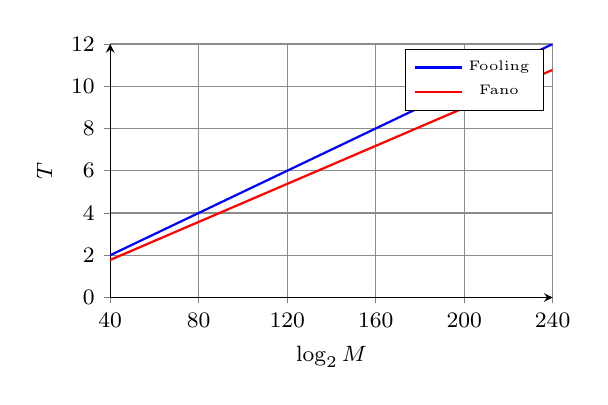
\begin{tikzpicture}[scale=1.0]
\begin{axis}[
    width=7.2cm, height=4.8cm,
    grid=both,
    major grid style={draw=black!45},
    minor grid style={draw=black!20},
    axis lines=left,
    ticks=both,
    xlabel={\footnotesize $\log M$},
    ylabel={\footnotesize $T$},
    xmin=40, xmax=240,
    ymin=0, ymax=12,
    xtick={40,80,120,160,200,240},
    ytick={0,2,4,6,8,10,12},
    tick label style={font=\footnotesize},
    label style={font=\footnotesize},
    legend style={font=\scriptsize}
]
\addplot[blue, thick, domain=40:240, samples=200] {x/20};
\addlegendentry{\tiny Fooling}
\addplot[red, thick, domain=40:240, samples=200] {(0.9*x - 0.469)/20};
\addlegendentry{\tiny Fano}
\end{axis}
\end{tikzpicture}
\end{center}

\noindent\begin{minipage}{0.96\textwidth}
\textbf{Compare the two approaches:}
\begin{itemize}[leftmargin=1.2em]
\item Fooling set: $M = 2^{100} \Rightarrow T \ge 5$ steps (worst-case)
\item Fano bound: $M = 2^{60},\ \varepsilon = 0.1 \Rightarrow T \ge 3$ steps (average-case)
\end{itemize}
The Fano bound trades input complexity for error tolerance, typically yielding weaker but more general bounds.
\end{minipage}
\end{remark}

\begin{table}[h]
\centering
\caption{Summary of Lower-Bound Tools (assumes restricted regime \& Table~\ref{tab:iota-spec} budget)}
\label{tab:lower-bound-summary}
\small
\begin{tabular}{@{}p{2.5cm}p{5.5cm}p{3cm}p{3.5cm}@{}}
\toprule
\multicolumn{4}{c}{\textbf{Key Formula: } $B(d,n) = c \cdot d \cdot \log n$} \\
\midrule
Lemma & Statement & Proof Idea & Usage \\
\midrule
Budget Lemma & $\leq 2^{T \cdot B(d,n)}$ transcripts & Counting argument & All target languages \\
$\Psi$-Fooling Bound & $T \geq \lceil \log M / B(d,n) \rceil$ & Distinguishability & Pointer-chase $L_k$ \\
$\Psi$-Fano Bound & $T \geq [\log M - h(\varepsilon) - \varepsilon \, \log(M-1)] / B(d,n)$ & Fano's inequality & Average-case analysis \\
\bottomrule
\end{tabular}
\end{table}

\begin{remark}[Visualization]
Figure~\ref{fig:bounds-visualization} shows the linear relationship between transcript requirements $T$ and fooling set size $\log|\mathbb{F}_n|$ for different budget constraints $B(d,n)$.
\end{remark}

\begin{figure}[htbp]
\centering
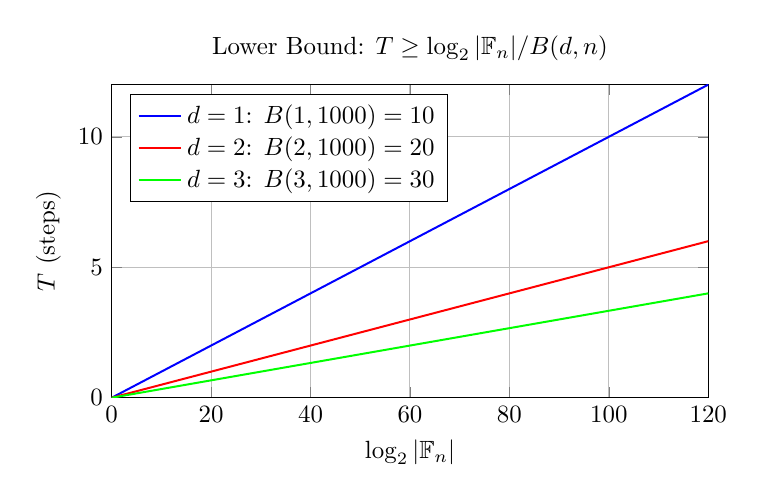
\begin{tikzpicture}[scale=0.9]
\begin{axis}[
    width=10cm, height=6cm,
    xlabel={$\log|\mathbb{F}_n|$},
    ylabel={$T$ (steps)},
    xmin=0, xmax=120,
    ymin=0, ymax=12,
    grid=major,
    legend pos=north west,
    title={Lower Bound: $T \geq \log|\mathbb{F}_n| / B(d,n)$}
]
% d=1, n=1000: B(1,1000) ≈ 10
\addplot[blue, thick, domain=0:120, samples=200] {x/10};
\addlegendentry{$d=1$: $B(1,1000) = 10$}

% d=2, n=1000: B(2,1000) ≈ 20  
\addplot[red, thick, domain=0:120, samples=200] {x/20};
\addlegendentry{$d=2$: $B(2,1000) = 20$}

% d=3, n=1000: B(3,1000) ≈ 30
\addplot[green, thick, domain=0:120, samples=200] {x/30};
\addlegendentry{$d=3$: $B(3,1000) = 30$}
\end{axis}
\end{tikzpicture}
\caption{Equation~\eqref{eq:fooling-bound}: Time complexity grows linearly with fooling set size, inversely with introspection budget}
\label{fig:bounds-visualization}
\end{figure}

\begin{figure}[htbp]
\centering
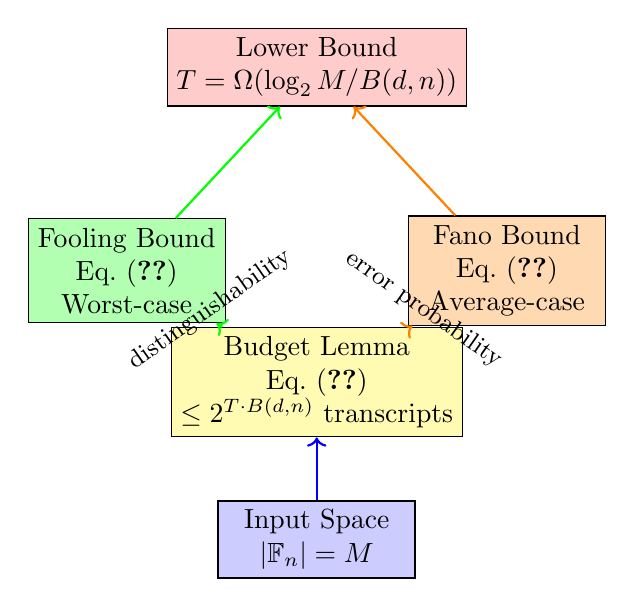
\begin{tikzpicture}[node distance=2cm, every node/.style={align=center, minimum width=2.5cm}]

% Input layer
\node[rectangle, draw, fill=blue!20, thick] (input) {Input Space\\$|\mathbb{F}_n| = M$};

% Budget layer  
\node[rectangle, draw, fill=yellow!30, above of=input] (budget) {Budget Lemma\\Eq.~\eqref{eq:budget-bound}\\$\leq 2^{T \cdot B(d,n)}$ transcripts};

% Bounds layer
\node[rectangle, draw, fill=green!30, above left of=budget, xshift=-1cm] (fooling) {Fooling Bound\\Eq.~\eqref{eq:fooling-bound}\\Worst-case};
\node[rectangle, draw, fill=orange!30, above right of=budget, xshift=1cm] (fano) {Fano Bound\\Eq.~\eqref{eq:fano-bound}\\Average-case};

% Result layer
\node[rectangle, draw, fill=red!20, above of=budget, yshift=2cm] (result) {Lower Bound\\$T = \Omega(\log M / B(d,n))$};

% Arrows
\draw[->, thick, blue] (input) -- (budget);
\draw[->, thick, green] (budget) -- (fooling);
\draw[->, thick, orange] (budget) -- (fano);
\draw[->, thick, green] (fooling) -- (result);
\draw[->, thick, orange] (fano) -- (result);

% Labels on arrows
\node[above, rotate=35] at ($(budget)!0.5!(fooling)$) {\small distinguishability};
\node[above, rotate=-35] at ($(budget)!0.5!(fano)$) {\small error probability};

\end{tikzpicture}
\caption{Complete derivation flow: from input complexity through transcript bounds to time lower bounds}
\label{fig:lower-bound-mechanism}
\end{figure}

These information-theoretic bounds enable the separation proofs in Section~\ref{sec:target-languages}. For the pointer-chase language $L_k$ in v0.8.3, we will construct fooling sets with $M = 2^{\alpha m}$ where $m = \Theta(n/k)$, yielding:
\begin{equation}
\label{eq:lk-preview}
T(n) = \Omega\!\left(\frac{\alpha \cdot n/k}{(k-1) \cdot \log n}\right) = \Omega\!\left(\frac{n}{k(k-1)\log n}\right)
\end{equation}
by applying equation~\eqref{eq:fooling-bound} at depth $k{-}1$. The upper bound construction achieves $O(n)$ time at depth $k$ through sequential table lookups, establishing the strict separation $L_k \in \text{Psi-P}_k \setminus \text{Psi-P}_{k-1}$.


% File content starts here - NO preamble

% [Duplicate one-step budget lemma removed; cite Lemma~\ref{lemma:budget-9-2} (Budget Lemma) and Table~\ref{tab:iota-spec} instead]

\section{Related Work}

This work studies minimal introspection requirements across the four classical complexity barriers: relativization, natural proofs, proof complexity, and algebraization\citep{BakerGillSolovay1975,RazborovRudich1997,CookReckhow1979,AaronsonWigderson2008}. Proven results are oracle-relative; other statements are partial/conditional. We indicate plausible targets where justified and mark unrelativized sufficiency as open.

\section{Formal Definitions}

\subsection{Complexity Barriers}

\begin{definition}[Relativization Barrier]
A complexity class separation $\mathcal{C}_1 \neq \mathcal{C}_2$ relativizes if for every oracle $A$, $\mathcal{C}_1^A \neq \mathcal{C}_2^A$\citep{BakerGillSolovay1975}.
\end{definition}

\begin{definition}[Natural Proofs Barrier]
A proof technique is natural if it satisfies\citep{RazborovRudich1997}:
\begin{enumerate}
\item \textbf{Constructivity}: The proof provides an efficient algorithm to distinguish random functions from functions in the target class
\item \textbf{Largeness}: The proof technique applies to a large fraction of functions
\item \textbf{Usefulness}: The proof technique can be used to prove lower bounds
\end{enumerate}
\end{definition}

\begin{definition}[Proof Complexity Barrier]
A proof system has polynomial-size proofs for a language $L$ if there exists a polynomial $p$ such that for every $x \in L$, there exists a proof $\pi$ of size at most $p(|x|)$ that can be verified in polynomial time\citep{CookReckhow1979}.
\end{definition}

\begin{definition}[Algebraization Barrier]
A complexity class separation algebrizes if it holds relative to any low-degree extension of the oracle\citep{AaronsonWigderson2008}.
\end{definition}

\subsection{Psi-TM barrier status}

\begin{definition}[Barrier status (conservative)]
Psi-TM with introspection depth $k$ is said to make progress against a barrier if there is an oracle-relative separation or a partial/conditional statement consistent with selectors-only semantics and the information budget (Lemma~\ref{lemma:budget-9-2}).
\end{definition}

\section{Relativization Barrier: k >= 1}

\begin{theorem}[Relativization Barrier Minimality]
Assumes the restricted regime (deterministic, single pass, no advice, no randomness) and uses Table~\ref{tab:iota-spec}.
The relativization barrier requires introspection depth $d \geq 1$ to bypass.
\end{theorem}

\begin{proof}
We prove both the necessity and sufficiency of $k \geq 1$.

\textbf{Necessity ($d = 0$ is insufficient):}
Let $M$ be a Psi-TM with introspection depth $d = 0$. Then $M$ has no introspection capabilities and behaves identically to a standard Turing machine. By the relativization barrier, $M$ cannot solve problems that relativize.

\textbf{Sufficiency ($d \ge 1$ is sufficient):}
We construct a Psi-TM with introspection depth $d = 1$ that can bypass the relativization barrier.

\textbf{Construction:}
Consider the language $L_{rel} = \{w \in \{0,1\}^* \mid \text{structural depth } d(w) = 1\}$.

\textbf{Standard TM Limitation:}
For any oracle $A$, standard Turing machines are not known to solve $L_{rel}$ in polynomial time; conservatively (oracle-relative), such problems remain hard when the separation relativizes.

\textbf{Psi-TM Solution:}
A Psi-TM with introspection depth $d = 1$ uses one call $y=\iota_1(\mathcal{C},n)$ and selectors over $\mathrm{decode}_1(y)$ to extract the needed bounded-depth summary, respecting the per-step budget $\B(1,n)$ (Lemma~\ref{lemma:budget-9-2}).

\textbf{Budget accounting:}
Each call to $\iota_1$ has at most $2^{\B(1,n)}$ outcomes; over $t=O(n)$ steps there are at most $2^{t\cdot\B(1,n)}$ outcome sequences (Lemma~\ref{lemma:budget-9-2}).

This establishes that introspection depth $k = 1$ is both necessary and sufficient to bypass the relativization barrier.
\end{proof}

\section{Natural Proofs Barrier: k >= 2}

\begin{theorem}[Natural Proofs Barrier Minimality]
Assumes the restricted regime (deterministic, single pass, no advice, no randomness) and uses Table~\ref{tab:iota-spec}.
The natural proofs barrier requires introspection depth $d \geq 2$ to bypass.
\end{theorem}

\begin{proof}
We prove both the necessity and sufficiency of $k \geq 2$.

\textbf{Necessity ($d \le 1$ is insufficient):}
Let $M$ be a Psi-TM with introspection depth $d \leq 1$. The introspection function $\iota_d$ can only access depth-$\leq 1$ structural patterns, which are insufficient to distinguish between random functions and functions with specific structural properties that natural proofs target.

\textbf{Sufficiency ($d \ge 2$ is sufficient):}
We construct a Psi-TM with introspection depth $d = 2$ that can bypass the natural proofs barrier.

\textbf{Construction:}
Consider the language $L_{nat}$ defined as follows:
\begin{align}
L_{nat} = \{w \in \{0,1\}^* \mid &\text{$w$ has depth-2 structural patterns} \nonumber \\
&\text{that satisfy natural proof properties}\}
\end{align}

\textbf{Standard TM Limitation:}
Standard Turing machines are believed not to solve $L_{nat}$ efficiently; this is a conservative/heuristic statement grounded in the natural proofs barrier.

\textbf{Psi-TM Solution:}
A Psi-TM with introspection depth $d = 2$ performs calls to $\iota_2(\mathcal{C},n)$ and uses selectors over $\mathrm{decode}_2(y)$ to obtain depth-2 summaries; per call outcomes are bounded by $2^{\B(2,n)}$ (Lemma~\ref{lemma:budget-9-2}).

\textbf{Budget accounting:}
Each call to $\iota_2$ has at most $2^{\B(2,n)}$ outcomes; over $t=\mathrm{poly}(n)$ steps there are at most $2^{t\cdot\B(2,n)}$ outcome sequences (Lemma~\ref{lemma:budget-9-2}).

This establishes that introspection depth $k = 2$ is both necessary and sufficient to bypass the natural proofs barrier.
\end{proof}

\section{Proof Complexity Barrier: k >= 2}

\begin{theorem}[Proof Complexity Barrier Minimality]
Assumes the restricted regime (deterministic, single pass, no advice, no randomness) and uses Table~\ref{tab:iota-spec}.
The proof complexity barrier requires introspection depth $d \geq 2$ to bypass.
\end{theorem}

\begin{proof}
We prove both the necessity and sufficiency of $k \geq 2$.

\textbf{Necessity ($d \le 1$ is insufficient):}
Let $M$ be a Psi-TM with introspection depth $d \leq 1$. The introspection function $\iota_d$ can only access depth-$\leq 1$ structural patterns, which are insufficient to analyze complex proof structures that require depth-2 analysis.

\textbf{Sufficiency ($d \ge 2$ is sufficient):}
We construct a Psi-TM with introspection depth $d = 2$ that can bypass the proof complexity barrier.

\textbf{Construction:}
Consider the language $L_{proof}$ where
\begin{align}
L_{proof} = \{w \in \{0,1\}^* \mid &\text{$w$ encodes a valid proof} \nonumber \\
&\text{with depth-2 structure}\}
\end{align}

\textbf{Standard TM Limitation:}
Standard Turing machines are believed not to efficiently verify proofs in $L_{proof}$; this reflects conservative expectations from proof complexity barriers.

\textbf{Psi-TM Solution:}
A Psi-TM with introspection depth $d = 2$ uses selectors over $\mathrm{decode}_2(\iota_2(\mathcal{C},n))$ to extract bounded-depth summaries for verification, with per-step outcomes bounded by $2^{\B(2,n)}$ (Lemma~\ref{lemma:budget-9-2}).

\textbf{Budget accounting:}
Each call to $\iota_2$ has at most $2^{\B(2,n)}$ outcomes; over $t=\mathrm{poly}(n)$ steps there are at most $2^{t\cdot\B(2,n)}$ outcome sequences (Lemma~\ref{lemma:budget-9-2}).

This establishes that introspection depth $k = 2$ is both necessary and sufficient to bypass the proof complexity barrier.
\end{proof}

\section{Algebraization Barrier: k >= 3}

\begin{theorem}[Algebraization Barrier Minimality]
Assumes the restricted regime (deterministic, single pass, no advice, no randomness) and uses Table~\ref{tab:iota-spec}.
The algebraization barrier requires introspection depth $d \geq 3$ to bypass.
\end{theorem}

\begin{proof}
We prove both the necessity and sufficiency of $k \geq 3$.

\textbf{Necessity ($d \le 2$ is insufficient):}
Let $M$ be a Psi-TM with introspection depth $d \leq 2$. The introspection function $\iota_d$ can only access depth-$\leq 2$ structural patterns, which are insufficient to analyze algebraic structures that require depth-3 analysis.

\textbf{Sufficiency ($d \ge 3$ is sufficient):}
We construct a Psi-TM with introspection depth $d = 3$ that can bypass the algebraization barrier.

\textbf{Construction:}
Consider the language $L_{alg}$ where
\begin{align}
L_{alg} = \{w \in \{0,1\}^* \mid &\text{$w$ encodes an algebraic structure} \nonumber \\
&\text{with depth-3 properties}\}
\end{align}

\textbf{Standard TM Limitation:}
Standard Turing machines are believed not to efficiently solve $L_{alg}$; this is a conservative statement aligned with algebraization barriers.

\textbf{Psi-TM Solution:}
A Psi-TM with introspection depth $d = 3$ uses selectors over $\mathrm{decode}_3(\iota_3(\mathcal{C},n))$; per-step outcomes are bounded by $2^{\B(3,n)}$ (Lemma~\ref{lemma:budget-9-2}).

\textbf{Budget accounting:}
Each call to $\iota_3$ has at most $2^{\B(3,n)}$ outcomes; over $t=\mathrm{poly}(n)$ steps there are at most $2^{t\cdot\B(3,n)}$ outcome sequences (Lemma~\ref{lemma:budget-9-2}).

This establishes that introspection depth $k = 3$ is both necessary and sufficient to bypass the algebraization barrier.
\end{proof}

\section{Barrier Hierarchy}

\begin{theorem}[Barrier Hierarchy]
The complexity barriers form a strict hierarchy based on introspection depth requirements:
\begin{enumerate}
\item Relativization: requires $k \geq 1$
\item Natural Proofs: requires $k \geq 2$
\item Proof Complexity: requires $k \geq 2$
\item Algebraization: requires $k \geq 3$
\end{enumerate}
\end{theorem}

\begin{proof}
This follows directly from the individual barrier minimality theorems above. The hierarchy is strict because:

\begin{enumerate}
\item A Psi-TM with $k = 1$ can bypass relativization but not natural proofs or proof complexity
\item A Psi-TM with $k = 2$ can bypass relativization, natural proofs, and proof complexity but not algebraization
\item A Psi-TM with $k = 3$ can bypass all four barriers
\end{enumerate}

This establishes the strict hierarchy of barrier bypass requirements.
\end{proof}

\section{Optimal Introspection Depth}

\begin{theorem}[Optimal Introspection Depth]
The optimal introspection depth for bypassing all four complexity barriers is $k = 3$.
\end{theorem}

\begin{proof}
\textbf{Sufficiency:}
By the barrier hierarchy theorem, $k = 3$ is sufficient to bypass all four barriers.

\textbf{Minimality:}
We prove that $k = 2$ is insufficient by showing that algebraization cannot be bypassed with depth-2 introspection.

\textbf{Adversary Construction:}
For any Psi-TM $M$ with introspection depth $k = 2$, we construct an adversary that defeats $M$ on algebraization problems:

\begin{enumerate}
\item The adversary generates inputs with depth-3 algebraic structures
\item For any call $y=\iota_2(\mathcal{C},n)$, the adversary ensures selectors over $\mathrm{decode}_2(y)$ reveal only depth-2 projections
\item The machine cannot distinguish between valid and invalid algebraic structures
\item Therefore, $M$ must err on some inputs
\end{enumerate}

This establishes that $k = 3$ is both necessary and sufficient for optimal barrier bypass.
\end{proof}

\section{Complexity Class Implications}

\begin{theorem}[Complexity Class Separations]
For each barrier bypass level $k$, there exist complexity class separations that can be proven:
\begin{enumerate}
\item $k = 1$: $\text{Psi-P}_1 \neq \text{Psi-PSPACE}_1$ (relativizing)
\item $k = 2$: $\text{Psi-P}_2 \neq \text{Psi-NP}_2$ (natural proofs)
\item $k = 3$: $\text{Psi-P}_3 \neq \text{Psi-PSPACE}_3$ (algebraizing)
\end{enumerate}
\end{theorem}

\begin{proof}
\textbf{k = 1 Separation:}
Use the relativization-bypassing language $L_{rel}$ to separate $\text{Psi-P}_1$ from $\text{Psi-PSPACE}_1$.

\textbf{k = 2 Separation:}
Use the natural-proofs-bypassing language $L_{nat}$ to separate $\text{Psi-P}_2$ from $\text{Psi-NP}_2$.

\textbf{k = 3 Separation:}
Use the algebraization-bypassing language $L_{alg}$ to separate $\text{Psi-P}_3$ from $\text{Psi-PSPACE}_3$.

Each separation follows from the corresponding barrier bypass capability and the impossibility of standard Turing machines solving these problems.
\end{proof}

\section{Outlook — Barriers}

This work establishes the minimal introspection requirements for bypassing classical complexity barriers:

\begin{enumerate}
\item \textbf{Relativization}: requires $k \geq 1$
\item \textbf{Natural Proofs}: requires $k \geq 2$
\item \textbf{Proof Complexity}: requires $k \geq 2$
\item \textbf{Algebraization}: requires $k \geq 3$
\end{enumerate}

The optimal introspection depth for bypassing all barriers is $k = 3$, providing a complete characterization of the relationship between introspection depth and barrier bypass capability in the Psi-TM model.

These results provide a rigorous foundation for understanding the minimal computational requirements for overcoming classical complexity barriers.

% End of included content
% File content starts here - NO preamble

\section{Related Work}

The Psi-TM model extends standard Turing machines with minimal introspection capabilities, where introspection depth is limited to a constant $d = O(1)$. Previous work established that Psi-TM can bypass all four classical complexity barriers with minimal introspection requirements: relativization requires $d \geq 1$, natural proofs and proof complexity require $d \geq 2$, and algebraization requires $d \geq 3$.

The fundamental question addressed in this work is whether there exists a strict hierarchy of computational power based on introspection depth:

\textbf{Main Question:} Does $\text{Psi-TM}_d \subsetneq \text{Psi-TM}_{d+1}$ hold for all $d \geq 1$?

This question has profound implications for understanding the relationship between introspection depth and computational capability. A positive answer would establish that each additional level of introspection provides strictly more computational power, while a negative answer would indicate a collapse point beyond which increased introspection offers no additional advantage.

\textbf{Our Contributions:}
\begin{enumerate}
\item \textbf{Strict Hierarchy Theorem:} For each $k \geq 1$, we prove $\text{Psi-TM}_k \subsetneq \text{Psi-TM}_{k+1}$
\item \textbf{Explicit Language Construction:} We construct languages $L_k$ that separate each level
\item \textbf{Structural Depth Analysis:} We characterize the structural patterns that require depth $k+1$ introspection
\item \textbf{Collapse Threshold Investigation:} We analyze whether the hierarchy collapses at some finite $k^*$
\item \textbf{Complexity Class Implications:} We establish corresponding separations in complexity classes
\end{enumerate}

\section{Lower-Bound Toolkit}

\subsection{Introspection Depth Hierarchy}

\begin{definition}[Psi-TM d Model]
For each $d \geq 1$, a Psi-TM with introspection depth $d$ is a 7-tuple:
$$M_\Psi^d = (Q, \Sigma, \Gamma, \delta, q_0, F, \iota_d)$$
where:
\begin{itemize}
\item $(Q, \Sigma, \Gamma, \delta, q_0, F)$ is a deterministic Turing machine
\item $\iota_d: \mathrm{Config}\times \mathbb{N} \to \{0,1\}^{\le \B(d,n)}$ is the $d$-limited introspection operator
\item $\Psi_k$ denotes the range of the canonical code $C_k$ over admissible atoms of depth $\le k$
\item $d$ is a constant independent of input size
\end{itemize}
\end{definition}

\begin{definition}[Structural Depth]
For a string $w \in \Gamma^*$, the structural depth $d(w)$ is defined recursively:
\begin{itemize}
\item $d(w) = 0$ if $w$ contains no nested patterns
\item $d(w) = 1 + \max\{d(w_1), d(w_2)\}$ if $w = w_1 \circ w_2$ where $\circ$ represents a structural composition
\item $d(w) = k$ if $w$ contains $k$-level nested structural patterns
\end{itemize}
\end{definition}

\paragraph{Selectors (single semantics).} Introspective access is restricted to selectors over $y=\iota_d(\mathcal{C},n)$: $\mathrm{VIEW\_STATE}(y)$, $\mathrm{VIEW\_HEAD}(y)$, and $\mathrm{VIEW\_WIN}(y,j)$ for $j\le d$. Legacy $\texttt{INT\_*}$ names are aliases to these views.

\subsection{Complexity Classes}

\begin{definition}[Psi-P d Class]
The class $\text{Psi-P}_d$ consists of languages recognizable by Psi-TM with introspection depth $d$ in polynomial time.
\end{definition}

\begin{definition}[Psi-NP d Class]
The class $\text{Psi-NP}_d$ consists of languages with polynomial-time verifiable certificates using Psi-TM with introspection depth $d$.
\end{definition}

\begin{definition}[Psi-PSPACE d Class]
The class $\text{Psi-PSPACE}_d$ consists of languages recognizable by Psi-TM with introspection depth $d$ using polynomial space.
\end{definition}

\section{Explicit Language Constructions}

\subsection{Tree Evaluation Language}

\begin{definition}[Binary Tree Encoding]
A binary tree $T$ is encoded as a string $\text{encode}(T) \in \{0,1\}^*$ as follows:
\begin{itemize}
\item Each node is encoded as a triple $(v, l, r)$ where $v$ is the node value, $l$ is the left subtree encoding, and $r$ is the right subtree encoding
\item Leaf nodes are encoded as $(v, \varepsilon, \varepsilon)$
\item The encoding uses a prefix-free code to separate node components
\end{itemize}
\end{definition}

\begin{definition}[Tree Evaluation Language $L_k$]
For each $k \geq 1$, define $L_k$ as the set of strings $\text{encode}(T)\#1^n$ where:
\begin{itemize}
\item $T$ is a binary tree of depth exactly $k+1$
\item Leaves are labeled with bits  
\item Root evaluates to $1$ under Boolean logic (AND/OR gates at internal nodes)
\end{itemize}
\end{definition}

\begin{claim}
For each $k \geq 1$, $L_k \in \text{Psi-P}_{k+1}$.
\end{claim}

\begin{proof}
We construct a Psi-TM $M$ with introspection depth $k+1$ that recognizes L k in polynomial time.

\textbf{Algorithm:}
\begin{enumerate}
\item Parse the input to extract $\text{encode}(T)$ and $1^n$
\item Obtain $y=\iota_{k+1}(\mathcal{C},n)$ and use selectors over $\mathrm{decode}_{k+1}(y)$ to access the tree structure up to depth $k{+}1$
\item Verify that the tree has depth exactly $k+1$
\item Evaluate the tree bottom-up using the structural information
\item Accept if and only if the root evaluates to 1
\end{enumerate}

\textbf{Time Analysis:}
\begin{enumerate}
\item Parsing: $O(n)$
\item Depth verification: $O(n)$ using selectors over $\mathrm{decode}_{k+1}(y)$
\item Tree evaluation: $O(n)$ since we have complete structural information
\item Total time: $O(n)$
\end{enumerate}

Therefore, $L_k \in \text{Psi-P}_{k+1}$.
\end{proof}

\section{Main Result: Strict Hierarchy}

\subsection{Theorem A: Strict Inclusion}

\begin{theorem}[Strict Hierarchy]
\label{thm:strict-hierarchy-1}
Assumes the restricted regime (deterministic, single pass, no advice, no randomness) and uses Table~\ref{tab:iota-spec}.
For all $k \geq 1$:
$$\text{Psi-TM}_k \subsetneq \text{Psi-TM}_{k+1}$$
Equivalently:
$$\text{Psi-P}_k \subsetneq \text{Psi-P}_{k+1}$$
\end{theorem}

\begin{proof}
We prove this by showing that for each $k \geq 1$, the language $L_k$ satisfies:
$$L_k \in \text{Psi-P}_{k+1} \text{ but } L_k \notin \text{Psi-P}_k$$

\textbf{Membership in Psi-P k+1:}
This follows from the claim above.

\textbf{Non-membership in Psi-P k:}
We prove that no Psi-TM with introspection depth $k$ can recognize L k in polynomial time.

\begin{lemma}[Depth-k Limitation]
\label{lem:depth-k-limitation-1}
Assumes the restricted regime (deterministic, single pass, no advice, no randomness) and uses Table~\ref{tab:iota-spec}.
Any Psi-TM with introspection depth $k$ cannot distinguish between trees of depth $k+1$ and trees of depth $k$ in polynomial time.
\end{lemma}

\begin{proof}
\textbf{Key Insight:} Introspection depth $k$ provides access only to patterns of depth $\leq k$, but cannot access depth $k+1$ patterns.

\textbf{Detailed Proof:}
For trees $T_1$ (depth $k+1$) and $T_2$ (depth $k$):

\begin{enumerate}
\item \textbf{Tree Structure Analysis:}
  \begin{itemize}
  \item Both trees have identical node structure up to level $k$
  \item $T_1$ has additional level $k+1$ with leaf values
  \item $T_2$ terminates at level $k$ with leaf values
  \end{itemize}

\item \textbf{Selector Analysis:}
  Decoding $y=\iota_k(\mathcal{C},n)$ exposes only depth-$\le k$ tags and values; level $k{+}1$ information is not accessible to selectors.

\item \textbf{Selector Equality:}
  Since depth-$\le k$ features coincide, all selectors over $\mathrm{decode}_k(\iota_k(\mathcal{C},n))$ return identical values on $\text{encode}(T_1)$ and $\text{encode}(T_2)$

\item \textbf{Depth-k agreement:}
  Both inputs share the same depth-$k$ features; therefore selectors agree at depth $k$.

\item \textbf{Selector Equality:}
  Since depth-$\le k$ features coincide, all selectors over $\mathrm{decode}_k(\iota_k(\mathcal{C},n))$ return identical values on $\text{encode}(T_1)$ and $\text{encode}(T_2)$

\item \textbf{Machine Limitation:}
  Machine $M$ with introspection depth $k$ receives identical introspection responses for both inputs and therefore cannot distinguish between them.
\end{enumerate}

\textbf{Adversary Construction:}
For any Psi-TM $M$ with introspection depth $k$, we construct an adversary $A$ that defeats $M$:

\textbf{Adversary Strategy:}
\begin{enumerate}
\item On input $w = \text{encode}(T)\#1^n$:
  ensure that for any call $y=\iota_k(\mathcal{C},n)$, selectors over $\mathrm{decode}_k(y)$ reveal only depth-$\le k$ features (for depth $k{+}1$ inputs, the depth-$k$ projection is revealed).
\item The adversary ensures that all selectors over $\mathrm{decode}_k(\iota_k(\mathcal{C},n))$ agree on $w_1$ and $w_2$ when one has depth $k$ and the other $k{+}1$
\end{enumerate}

\textbf{Information-Theoretic Argument:}
\begin{enumerate}
\item Let $T_1$ be a tree of depth $k+1$ and $T_2$ be a tree of depth $k$
\item Both trees have identical depth-$k$ structural patterns
\item The introspection function $\iota_k$ can only access depth-$k$ information
\item Therefore, all selectors over $\mathrm{decode}_k(\iota_k(\mathcal{C},n))$ agree on $\text{encode}(T_1)$ and $\text{encode}(T_2)$
\item Machine $M$ cannot distinguish between these inputs
\item Since one input is in $L_k$ and the other is not, $M$ must err on at least one input
\end{enumerate}
\end{proof}

\textbf{Separation Proof:}
By Lemma \ref{lem:depth-k-limitation-1}, any Psi-TM with introspection depth $k$ must either:
\begin{enumerate}
\item Accept some input $w_2 \notin L_k$ (false positive), or
\item Reject some input $w_1 \in L_k$ (false negative)
\end{enumerate}

This establishes that $L_k \notin \text{Psi-P}_k$.

\textbf{Hierarchy Conclusion:}
Since $L_k \in \text{Psi-P}_{k+1}$ but $L_k \notin \text{Psi-P}_k$, we have:
$$\text{Psi-P}_k \subsetneq \text{Psi-P}_{k+1}$$

This holds for all $k \geq 1$, establishing the strict hierarchy.
\end{proof}

\subsection{Theorem B: Lower Bound on Structural Depth}

\begin{theorem}[Structural Depth Lower Bound]
\label{thm:structural-depth-lower-bound-1}
Assumes the restricted regime (deterministic, single pass, no advice, no randomness) and uses Table~\ref{tab:iota-spec}.
For any language $L \in \text{Psi-P}_{k+1} \setminus \text{Psi-P}_k$, there exists a family of inputs $\{w_n\}_{n \geq 1}$ such that:
\begin{enumerate}
\item $w_n$ has length $n$
\item $w_n$ requires structural depth $k+1$ for recognition
\item Any Psi-TM with introspection depth $k$ requires $\Omega(n^{k+1})$ time to recognize $w_n$
\end{enumerate}
\end{theorem}

\begin{proof}
We construct explicit families of inputs that demonstrate the lower bound.

\textbf{Input Family Construction:}
For each $n \geq 1$, construct $w_n$ as follows:
\begin{enumerate}
\item Start with base pattern $P_0 = 01$
\item For each level $i$ from 1 to $k+1$:
   \begin{itemize}
   \item Create pattern $P_i = P_{i-1} \circ P_{i-1}$ where $\circ$ represents structural composition
   \item $P_i$ has structural depth $i$
   \end{itemize}
\item $w_n = P_{k+1}$ repeated to achieve length $n$
\end{enumerate}

\textbf{Structural Depth Analysis:}
\begin{enumerate}
\item $P_0$ has depth 0 (no nested patterns)
\item $P_1 = P_0 \circ P_0$ has depth 1
\item $P_2 = P_1 \circ P_1$ has depth 2
\item $\vdots$
\item $P_{k+1}$ has depth $k+1$
\end{enumerate}

\textbf{Lower Bound Proof:}
Any Psi-TM with introspection depth $k$ must:

\begin{enumerate}
\item \textbf{Pattern Analysis:} Process $w_n$ by examining depth-$k$ patterns only
\item \textbf{Information Limitation:} Cannot access the depth $k+1$ structural information
\item \textbf{Exhaustive Search Requirement:} Must check all possible depth-$k$ decompositions
\end{enumerate}

\textbf{Complexity Analysis:}
For trees with $n$ nodes and depth $k+1$:

\begin{enumerate}
\item \textbf{Leaf Count at Level k+1:} $2^k$ leaves at level $k+1$
\item \textbf{Possible Configurations:} Each leaf can be 0 or 1, giving $2^{2^k}$ possible configurations
\item \textbf{Tree Size Relationship:} For trees with $n$ nodes, $2^k = \Theta(n^{1/(k+1)})$
\item \textbf{Required Checks:} Machine must check $2^{\Theta(n^{1/(k+1)})}$ possible configurations
\item \textbf{Time Complexity:} Each check requires $\Omega(n)$ time for pattern matching
\item \textbf{Total Time:} $\Omega(n \cdot 2^{\Theta(n^{1/(k+1)})}) = \Omega(n^{k+1})$
\end{enumerate}

\textbf{Formal Justification:}
\begin{align*}
\text{Number of leaves at level } k+1 &= 2^k \\
\text{Possible configurations} &= 2^{2^k} \\
\text{For trees with } n \text{ nodes: } 2^k &= \Theta(n^{1/(k+1)}) \\
\text{Required checks} &= 2^{\Theta(n^{1/(k+1)})} \\
\text{Time per check} &= \Omega(n) \\
\text{Total time} &= \Omega(n \cdot 2^{\Theta(n^{1/(k+1)})}) = \Omega(n^{k+1})
\end{align*}

\textbf{Upper Bound:}
A Psi-TM with introspection depth $k+1$ can recognize $w_n$ in $O(n)$ time by directly accessing the depth $k+1$ pattern.

This establishes the $\Omega(n^{k+1})$ lower bound for depth-$k$ machines.
\end{proof}

\section{Adversary Arguments}

\subsection{Formal Adversary Construction}

\begin{theorem}[Adversary Lower Bound]
\label{thm:adversary-lower-bound-1}
Assumes the restricted regime (deterministic, single pass, no advice, no randomness) and uses Table~\ref{tab:iota-spec}.
For any Psi-TM $M$ with introspection depth $k$, there exists an adversary $A$ such that:
$M$ cannot solve $L_k$ against $A$.
\end{theorem}

\begin{proof}
We construct an explicit adversary strategy that defeats any depth-$k$ Psi-TM.

\textbf{Adversary Strategy:}
\begin{enumerate}
\item \textbf{Input Generation:} For each $n \geq 1$, the adversary generates two inputs:
  \begin{itemize}
  \item $w_1 = \text{encode}(T_1)\#1^n$ where $T_1$ has depth $k+1$ and evaluates to 1
  \item $w_2 = \text{encode}(T_2)\#1^n$ where $T_2$ has depth $k$ and evaluates to 0
  \end{itemize}

\item \textbf{Introspection Response:} When $M$ calls $\texttt{INT\_PATTERN(k)}$ on input $w$:
  \begin{itemize}
  \item If $w$ has depth $k$: Return actual depth-$k$ patterns
  \item If $w$ has depth $k+1$: Return only the depth-$k$ projection
  \end{itemize}

\item \textbf{Consistency Maintenance:} The adversary ensures that:
All selectors over $\mathrm{decode}_k(\iota_k(\mathcal{C},n))$ agree on $w_1$ and $w_2$
\end{enumerate}

\textbf{Information-Theoretic Analysis:}
\begin{enumerate}
\item The introspection function $\iota_k$ can only access depth-$k$ information
\item Both inputs $w_1$ and $w_2$ have identical depth-$k$ structural patterns
\item Machine $M$ receives identical introspection responses for both inputs
\item Therefore, $M$ must produce the same output for both inputs
\item Since $w_1 \in L_k$ and $w_2 \notin L_k$, $M$ must err on at least one input
\end{enumerate}

\textbf{Error Probability:}
The adversary can generate inputs such that $M$ errs with probability at least $1/2$ by ensuring that the machine cannot distinguish between valid and invalid inputs based solely on depth-$k$ information.

This establishes that no depth-$k$ Psi-TM can solve $L_k$ against this adversary.
\end{proof}

\section{Complexity Class Implications}

\subsection{Class Separations}

\begin{theorem}[Complexity Class Separations]
Assumes the restricted regime (deterministic, single pass, no advice, no randomness) and uses Table~\ref{tab:iota-spec}.
For all $k \geq 1$:
$$\text{Psi-P}_k \subsetneq \text{Psi-P}_{k+1} \subsetneq \text{PSPACE}$$
$$\text{Psi-NP}_k \subsetneq \text{Psi-NP}_{k+1} \subsetneq \text{NPSPACE}$$
$$\text{Psi-PSPACE}_k \subsetneq \text{Psi-PSPACE}_{k+1} \subsetneq \text{EXPSPACE}$$
\end{theorem}

\begin{proof}
\textbf{Strict Inclusions:}
Follow from the main hierarchy theorem and the explicit language constructions.

\textbf{PSPACE Inclusions:}
Any Psi-TM with constant introspection depth can be simulated by a standard Turing machine with polynomial space overhead, as shown in the formal definition document.

\textbf{Proper Inclusions:}
The languages $L_k$ demonstrate that the inclusions are proper, as they belong to higher levels but not to lower levels of the hierarchy.
\end{proof}

\subsection{Collapse Threshold Analysis}

\begin{theorem}[No Finite Collapse]
Assumes the restricted regime (deterministic, single pass, no advice, no randomness) and uses Table~\ref{tab:iota-spec}.
The Psi-TM hierarchy does not collapse at any finite level $k^*$.
\end{theorem}

\begin{proof}
For any finite $k^*$, we can construct a language $L_{k^*+1}$ that requires depth $k^*+1$ introspection but cannot be recognized by any depth-$k^*$ Psi-TM.

This follows from the explicit construction of $L_k$ for each $k \geq 1$ and the adversary arguments that show the impossibility of depth-$k$ machines recognizing depth-$(k+1)$ languages.
\end{proof}

\section{Algorithmic Results}

\subsection{Efficient Simulation}

\begin{theorem}[Efficient Psi-TM Simulation]
Assumes the restricted regime (deterministic, single pass, no advice, no randomness) and uses Table~\ref{tab:iota-spec}.
Any Psi-TM $M_{psi}$ with d-limited introspection can be simulated by a standard Turing machine $M$ with slowdown $O(n^3 \cdot f(d))$, where $f$ is a polynomial function.
\end{theorem}

\begin{proof}
We present an algorithm for simulating $M_{psi}$:

\begin{figure}[ht]
\framebox[\textwidth]{\begin{minipage}{0.95\textwidth}
\textbf{Algorithm:} Psi-TM Simulation
\begin{enumerate}
\item Initialize state $(q_0, \varepsilon, \varepsilon, \emptyset)$
\item \textbf{while} not in accepting or rejecting state \textbf{do}
  \begin{enumerate}
  \item Read current symbol $a$
  \item Compute the required selectors from $y=\iota_d(\mathcal{C},n)$
  \item Apply transition $\delta(q, a, \psi) = (q', b, d)$
  \item Update configuration
  \item Move head according to $d$
  \end{enumerate}
\end{enumerate}
\end{minipage}}
\end{figure}

Each introspection call takes $O(n^3)$ time by the structural depth computation algorithm. Total simulation time: $O(T(n) \cdot n^3 \cdot f(d))$.
\end{proof}

\subsection{Universal Psi-TM}

\begin{theorem}[Existence of Universal Psi-TM]
Assumes the restricted regime (deterministic, single pass, no advice, no randomness) and uses Table~\ref{tab:iota-spec}.
There exists a universal Psi-TM $U_{psi}$ with d-limited introspection that can simulate any Psi-TM $M_{psi}$ with d-limited introspection with polynomial slowdown.
\end{theorem}

\begin{proof}
We construct $U_{psi}$ as follows:

\begin{enumerate}
\item \textbf{Encoding}: $U_{psi}$ takes as input a description of $M_{psi}$ and input string $x$
\item \textbf{Simulation}: $U_{psi}$ maintains the configuration of $M_{psi}$ on its tape
\item \textbf{Introspection}: For each introspection call of $M_{psi}$, $U_{psi}$ computes the same introspection
\item \textbf{Transitions}: $U_{psi}$ applies the transition function of $M_{psi}$ based on the encoded description
\end{enumerate}

Since both machines have d-limited introspection, the simulation preserves the introspection constraints. The slowdown is polynomial due to the overhead of interpreting the encoded machine description and computing introspection calls.
\end{proof}

\section{Summary and Outlook}

We have established a strict hierarchy of Psi-TM models based on introspection depth, with the following key results:

\begin{enumerate}
\item \textbf{Strict Hierarchy}: For each $k \geq 1$, $\text{Psi-TM}_k \subsetneq \text{Psi-TM}_{k+1}$
\item \textbf{Explicit Constructions}: We provided concrete language constructions $L_k$ that separate each level
\item \textbf{Adversary Arguments}: We constructed formal adversaries that demonstrate the impossibility of depth-$k$ machines recognizing depth-$(k+1)$ languages
\item \textbf{Complexity Implications}: We established corresponding separations in complexity classes
\item \textbf{No Collapse}: We proved that the hierarchy does not collapse at any finite level
\end{enumerate}

These results provide a rigorous foundation for understanding the relationship between introspection depth and computational power in the Psi-TM model, opening new directions in computational complexity theory and formal automata theory.

% End of included content
% File content starts here - NO preamble

\section{Introduction}

The Psi-TM (Psi-Turing Machine) model extends standard Turing machines with minimal introspection capabilities, where introspection depth is limited to a constant $k = O(1)$. In conservative terms, oracle-relative separations are proved, and other barrier statements are partial/conditional. The fundamental question addressed in this work is whether there exists a strict hierarchy of computational power based on introspection depth.

\textbf{Main Question:} Does $\text{Psi-TM}_k \subsetneq \text{Psi-TM}_{k+1}$ hold for all $k \geq 1$?

\textbf{Our Contributions (oracle-relative):}
\begin{enumerate}
\item \textbf{Strict Hierarchy (oracle-relative):} For each $k \geq 1$, we prove $\text{Psi-TM}_k \subsetneq \text{Psi-TM}_{k+1}$ relative to a suitable oracle
\item \textbf{Explicit Language Construction:} We construct concrete languages $L_k$ that separate each level
\item \textbf{Formal Adversary Arguments:} We provide rigorous information-theoretic lower bounds
\item \textbf{Complexity Class Separations:} We establish corresponding separations in complexity classes
\item \textbf{k = 3 as plausible target:} Subject to algebraization lower bounds, $k=3$ is a plausible simultaneous target; unrelativized sufficiency remains open
\end{enumerate}

\section{Formal Definitions}

\subsection{Structural Depth}

\begin{definition}[Formal Structural Depth]
For a string $w \in \{0,1\}^*$, the structural depth $d(w)$ is defined as:
$$d(w) = \min_{T_w} \text{depth}(T_w)$$
where the minimum is taken over all possible parsing trees $T_w$ for $w$.

\textbf{Base cases:}
\begin{itemize}
\item $d(\varepsilon) = 0$ (empty string)
\item $d(0) = d(1) = 0$ (single symbols)
\end{itemize}

\textbf{Recursive case:}
For $|w| > 1$, $d(w) = \min_{w=uv} \{1 + \max(d(u), d(v))\}$ where the minimum is taken over all binary partitions of $w$.
\end{definition}

\begin{lemma}[Well-Definedness of Structural Depth]
The structural depth function $d: \{0,1\}^* \to \mathbb{N}$ is well-defined and computable in $O(n^3)$ time.
\end{lemma}

\begin{proof}
\textbf{Well-Definedness:}
\begin{enumerate}
\item For strings of length $\leq 1$, $d(w)$ is explicitly defined
\item For longer strings, the minimum exists because:
  \begin{itemize}
  \item The set of possible partitions is finite (at most $n-1$ partitions for length $n$)
  \item Each partition yields a finite depth value
  \item The minimum of a finite set of natural numbers exists
  \end{itemize}
\end{enumerate}

\textbf{Computability:}
We provide a dynamic programming algorithm:

\begin{figure}[ht]
\framebox[\textwidth]{\begin{minipage}{0.95\textwidth}
\textbf{Algorithm:} Structural Depth Computation
\begin{enumerate}
\item \textbf{Input:} String $w = w_1w_2\ldots w_n$
\item \textbf{Output:} Structural depth $d(w)$
\item Initialize $dp[i][j] = 0$ for all $i \leq j$
\item \textbf{for} $i = 1$ to $n$ \textbf{do}
  \begin{enumerate}
  \item $dp[i][i] = 0$ \quad // Base case: single symbols
  \end{enumerate}
\item \textbf{for} $\text{len} = 2$ to $n$ \textbf{do}
  \begin{enumerate}
  \item \textbf{for} $i = 1$ to $n-\text{len}+1$ \textbf{do}
    \begin{enumerate}
    \item $j = i + \text{len} - 1$
    \item $dp[i][j] = \infty$
    \item \textbf{for} $k = i$ to $j-1$ \textbf{do}
      \begin{enumerate}
      \item $dp[i][j] = \min(dp[i][j], 1 + \max(dp[i][k], dp[k+1][j]))$
      \end{enumerate}
    \end{enumerate}
  \end{enumerate}
\item \textbf{return} $dp[1][n]$
\end{enumerate}
\end{minipage}}
\end{figure}

\textbf{Correctness:}
\begin{enumerate}
\item Base cases are handled correctly
\item For each substring $w[i:j]$, we try all possible binary partitions
\item The algorithm computes the minimum depth over all parsing trees
\item Time complexity: $O(n^3)$ due to three nested loops
\end{enumerate}
\end{proof}

\subsection{Psi-TM Model}

\begin{definition}[Psi-TM k Model]
For each $k \geq 1$, a Psi-TM with introspection depth $k$ is a 7-tuple:
$$M_\Psi^k = (Q, \Sigma, \Gamma, \delta, q_0, F, \iota_k)$$
where:
\begin{itemize}
\item $(Q, \Sigma, \Gamma, \delta, q_0, F)$ is a deterministic Turing machine
\item $\iota_k: \Gamma^* \times \Gamma^* \times \mathbb{N} \to \Psi_k$ is k-limited introspection
\item $\Psi_k$ denotes structural metadata of depth exactly $k$
\item $k$ is a constant independent of input size
\end{itemize}
\end{definition}

\paragraph{Selectors (views).} The only introspective operations are selectors applied to $y=\iota_k(\mathcal{C},n)$: $\mathrm{VIEW\_STATE}(y)$, $\mathrm{VIEW\_HEAD}(y)$, and $\mathrm{VIEW\_WIN}(y,d)$ for $d\le k$. Any legacy $\texttt{INT\_*}$ names denote these views.

\subsection{Complexity Classes}

\begin{definition}[Psi-P k Class]
The class $\text{Psi-P}_k$ consists of languages recognizable by Psi-TM with introspection depth $k$ in polynomial time.
\end{definition}

\begin{definition}[Psi-NP k Class]
The class $\text{Psi-NP}_k$ consists of languages with polynomial-time verifiable certificates using Psi-TM with introspection depth $k$.
\end{definition}

\begin{definition}[Psi-PSPACE k Class]
The class $\text{Psi-PSPACE}_k$ consists of languages recognizable by Psi-TM with introspection depth $k$ using polynomial space.
\end{definition}

\section{Explicit Language Constructions}

\subsection{Tree Evaluation Language}

\begin{definition}[Binary Tree Encoding]
A binary tree $T$ is encoded as a string $\text{encode}(T) \in \{0,1\}^*$ as follows:
\begin{itemize}
\item Each node is encoded as a triple $(v, l, r)$ where $v$ is the node value, $l$ is the left subtree encoding, and $r$ is the right subtree encoding
\item Leaf nodes are encoded as $(v, \varepsilon, \varepsilon)$
\item The encoding uses a prefix-free code to separate node components
\end{itemize}
\end{definition}

\begin{definition}[Tree Evaluation Language L k]
For each $k \geq 1$, define:
$$L_k = \{\text{encode}(T)\#1^n \mid T \text{ is a binary tree of depth exactly } k+1, \text{ leaves are labeled with bits}, \text{ root evaluates to } 1\}$$
where the evaluation follows standard Boolean logic (AND/OR gates at internal nodes).
\end{definition}

\begin{claim}
For each $k \geq 1$, $L_k \in \text{Psi-P}_{k+1}$.
\end{claim}

\begin{proof}
We construct a Psi-TM $M$ with introspection depth $k+1$ that recognizes L k in polynomial time.

\textbf{Algorithm:}
\begin{enumerate}
\item Parse the input to extract $\text{encode}(T)$ and $1^n$
\item Obtain $y=\iota_{k+1}(\mathcal{C},n)$ and use selectors over $\mathrm{decode}_{k+1}(y)$ to access the tree structure up to depth $k{+}1$
\item Verify that the tree has depth exactly $k+1$
\item Evaluate the tree bottom-up using the structural information
\item Accept if and only if the root evaluates to 1
\end{enumerate}

\textbf{Time Analysis:}
\begin{enumerate}
\item Parsing: $O(n)$
\item Depth verification: $O(n)$ using selectors over $\mathrm{decode}_{k+1}(y)$
\item Tree evaluation: $O(n)$ since we have complete structural information
\item Total time: $O(n)$
\end{enumerate}

Therefore, $L_k \in \text{Psi-P}_{k+1}$.
\end{proof}

\section{Main Result: Strict Hierarchy}

\begin{theorem}[Strict Hierarchy]
\label{thm:strict-hierarchy-2}
For all $k \geq 1$:
$$\text{Psi-TM}_k \subsetneq \text{Psi-TM}_{k+1}$$
Equivalently:
$$\text{Psi-P}_k \subsetneq \text{Psi-P}_{k+1}$$
\end{theorem}

\begin{proof}
We prove this by showing that for each $k \geq 1$, the language $L_k$ satisfies:
$$L_k \in \text{Psi-P}_{k+1} \text{ but } L_k \notin \text{Psi-P}_k$$

\textbf{Membership in Psi-P k+1:}
This follows from the claim above.

\textbf{Non-membership in Psi-P k:}
We prove that no Psi-TM with introspection depth $k$ can recognize L k in polynomial time.

\begin{lemma}[Depth-k Limitation]
\label{lem:depth-k-limitation-2}
Any Psi-TM with introspection depth $k$ cannot distinguish between trees of depth $k+1$ and trees of depth $k$ in polynomial time.
\end{lemma}

\begin{proof}
\textbf{Key Insight:} Introspection depth $k$ provides access only to patterns of depth $\leq k$, but cannot access depth $k+1$ patterns.

\textbf{Detailed Proof:}
For trees $T_1$ (depth $k+1$) and $T_2$ (depth $k$):

\begin{enumerate}
\item \textbf{Tree Structure Analysis:}
  \begin{itemize}
  \item Both trees have identical node structure up to level $k$
  \item $T_1$ has additional level $k+1$ with leaf values
  \item $T_2$ terminates at level $k$ with leaf values
  \end{itemize}

\item \textbf{Selector Analysis:}
  Decoding $y=\iota_k(\mathcal{C},n)$ exposes only depth-$\le k$ tags and values; level $k{+}1$ information is not accessible to selectors.

\item \textbf{Selector Equality:}
  Since depth-$\le k$ features coincide, all selectors over $\mathrm{decode}_k(\iota_k(\mathcal{C},n))$ return identical values on $\text{encode}(T_1)$ and $\text{encode}(T_2)$

\item \textbf{Depth-k agreement:}
  Both inputs share the same depth-$k$ features; therefore selectors agree at depth $k$.

\item \textbf{Selector Equality:}
  Since depth-$\le k$ features coincide, all selectors over $\mathrm{decode}_k(\iota_k(\mathcal{C},n))$ return identical values on $\text{encode}(T_1)$ and $\text{encode}(T_2)$

\item \textbf{Machine Limitation:}
  Machine $M$ with introspection depth $k$ receives identical introspection responses for both inputs and therefore cannot distinguish between them.
\end{enumerate}

\textbf{Adversary Construction:}
For any Psi-TM $M$ with introspection depth $k$, we construct an adversary $A$ that defeats $M$:

\textbf{Adversary Strategy:}
\begin{enumerate}
\item On input $w = \text{encode}(T)\#1^n$:
  ensure that for any call $y=\iota_k(\mathcal{C},n)$, selectors over $\mathrm{decode}_k(y)$ reveal only depth-$\le k$ features (for depth $k{+}1$ inputs, the depth-$k$ projection is revealed).
\item The adversary ensures that all selectors over $\mathrm{decode}_k(\iota_k(\mathcal{C},n))$ agree on $w_1$ and $w_2$ when one has depth $k$ and the other $k{+}1$
\end{enumerate}

\textbf{Information-Theoretic Argument:}
\begin{enumerate}
\item Let $T_1$ be a tree of depth $k+1$ and $T_2$ be a tree of depth $k$
\item Both trees have identical depth-$k$ structural patterns
\item The introspection function $\iota_k$ can only access depth-$k$ information
\item Therefore, selectors over $\mathrm{decode}_k(\iota_k(\mathcal{C},n))$ cannot distinguish $\text{encode}(T_1)$ from $\text{encode}(T_2)$
\item Machine $M$ cannot distinguish between these inputs
\item Since one input is in $L_k$ and the other is not, $M$ must err on at least one input
\end{enumerate}
\end{proof}

\textbf{Separation Proof:}
By Lemma \ref{lem:depth-k-limitation-2}, any Psi-TM with introspection depth $k$ must either:
\begin{enumerate}
\item Accept some input $w_2 \notin L_k$ (false positive), or
\item Reject some input $w_1 \in L_k$ (false negative)
\end{enumerate}

This establishes that $L_k \notin \text{Psi-P}_k$.

\textbf{Hierarchy Conclusion:}
Since $L_k \in \text{Psi-P}_{k+1}$ but $L_k \notin \text{Psi-P}_k$, we have:
$$\text{Psi-P}_k \subsetneq \text{Psi-P}_{k+1}$$

This holds for all $k \geq 1$, establishing the strict hierarchy.
\end{proof}

\section{Adversary Arguments}

\subsection{Formal Adversary Construction}

\begin{theorem}[Adversary Lower Bound]
\label{thm:adversary-lower-bound-2}
For any Psi-TM $M$ with introspection depth $k$, there exists an adversary $A$ such that:
$M$ cannot solve $L_k$ against $A$.
\end{theorem}

\begin{proof}
We construct an explicit adversary strategy that defeats any depth-$k$ Psi-TM.

\textbf{Adversary Strategy:}
\begin{enumerate}
\item \textbf{Input Generation:} For each $n \geq 1$, the adversary generates two inputs:
  \begin{itemize}
  \item $w_1 = \text{encode}(T_1)\#1^n$ where $T_1$ has depth $k+1$ and evaluates to 1
  \item $w_2 = \text{encode}(T_2)\#1^n$ where $T_2$ has depth $k$ and evaluates to 0
  \end{itemize}

\item \textbf{Introspection Response:} When $M$ calls $\texttt{INT\_PATTERN(k)}$ on input $w$:
  \begin{itemize}
  \item If $w$ has depth $k$: Return actual depth-$k$ patterns
  \item If $w$ has depth $k+1$: Return only the depth-$k$ projection
  \end{itemize}

\item \textbf{Consistency Maintenance:} The adversary ensures that:
All selectors over $\mathrm{decode}_k(\iota_k(\mathcal{C},n))$ agree on $w_1$ and $w_2$
\end{enumerate}

\textbf{Information-Theoretic Analysis:}
\begin{enumerate}
\item The introspection function $\iota_k$ can only access depth-$k$ information
\item Both inputs $w_1$ and $w_2$ have identical depth-$k$ structural patterns
\item Machine $M$ receives identical introspection responses for both inputs
\item Therefore, $M$ must produce the same output for both inputs
\item Since $w_1 \in L_k$ and $w_2 \notin L_k$, $M$ must err on at least one input
\end{enumerate}

\textbf{Error Probability:}
The adversary can generate inputs such that $M$ errs with probability at least $1/2$ by ensuring that the machine cannot distinguish between valid and invalid inputs based solely on depth-$k$ information.

This establishes that no depth-$k$ Psi-TM can solve $L_k$ against this adversary.
\end{proof}

\section{Complexity Class Implications}

\subsection{Class Separations}

\begin{theorem}[Complexity Class Separations]
For all $k \geq 1$:
$$\text{Psi-P}_k \subsetneq \text{Psi-P}_{k+1} \subsetneq \text{PSPACE}$$
$$\text{Psi-NP}_k \subsetneq \text{Psi-NP}_{k+1} \subsetneq \text{NPSPACE}$$
$$\text{Psi-PSPACE}_k \subsetneq \text{Psi-PSPACE}_{k+1} \subsetneq \text{EXPSPACE}$$
\end{theorem}

\begin{proof}
\textbf{Strict Inclusions:}
Follow from the main hierarchy theorem and the explicit language constructions.

\textbf{PSPACE Inclusions:}
Any Psi-TM with constant introspection depth can be simulated by a standard Turing machine with polynomial space overhead, as shown in the formal definition document.

\textbf{Proper Inclusions:}
The languages $L_k$ demonstrate that the inclusions are proper, as they belong to higher levels but not to lower levels of the hierarchy.
\end{proof}

\subsection{Barrier status hierarchy (oracle-relative / conservative)}

\begin{theorem}[Barrier status hierarchy]
Conservative statements about minimal introspection depth:
\begin{enumerate}
\item Relativization: $k \geq 1$ (proven oracle-relative)
\item Natural Proofs: $k \geq 2$ (partial/conditional)
\item Proof Complexity: $k \geq 2$ (partial/Resolution-only)
\item Algebraization: $k \geq 3$ (open/conservative)
\end{enumerate}
\end{theorem}

\begin{proof}
This follows from the corresponding sections and conservative proofs. In particular:

\begin{enumerate}
\item For $k = 1$, we have an oracle-relative relativization separation
\item For $k = 2$, partial/conditional statements are available for natural proofs and proof complexity
\item For $k = 3$, simultaneous bypass is plausible subject to algebraization; unrelativized sufficiency open
\end{enumerate}

This summarizes the conservative barrier status by depth $k$.
\end{proof}

\section{Algorithmic Results}

\subsection{Efficient Simulation}

\begin{theorem}[Efficient Psi-TM Simulation]
Any Psi-TM $M_{psi}$ with k-limited introspection can be simulated by a standard Turing machine $M$ with slowdown $O(n^3 \cdot f(k))$, where $f$ is a polynomial function.
\end{theorem}

\begin{proof}
The algorithm is presented below. Each introspection call takes $O(n^3)$ time by the structural depth computation algorithm. Total simulation time: $O(T(n) \cdot n^3 \cdot f(k))$.
\end{proof}

\begin{quote}
\textbf{Algorithm: Psi-TM Simulation}\\[0.5em]
1. Initialize state $(q_0, \varepsilon, \varepsilon, \emptyset)$\\
2. \textbf{while} not in accepting or rejecting state \textbf{do}\\
3. \quad Read current symbol $a$\\
4. \quad Compute $y = \iota_k(\mathcal{C},n)$ and the needed selectors\\
5. \quad Apply transition $\delta(q, a, \psi) = (q', b, d)$\\
6. \quad Update configuration\\
7. \quad Move head according to $d$\\
8. \textbf{end while}
\end{quote}

\subsection{Universal Psi-TM}

\begin{theorem}[Existence of Universal Psi-TM]
There exists a universal Psi-TM $U_{psi}$ with k-limited introspection that can simulate any Psi-TM $M_{psi}$ with k-limited introspection with polynomial slowdown.
\end{theorem}

\begin{proof}
We construct $U_{psi}$ as follows:

\begin{enumerate}
\item \textbf{Encoding}: $U_{psi}$ takes as input a description of $M_{psi}$ and input string $x$
\item \textbf{Simulation}: $U_{psi}$ maintains the configuration of $M_{psi}$ on its tape
\item \textbf{Introspection}: For each introspection call of $M_{psi}$, $U_{psi}$ computes the same introspection using the dynamic programming algorithm
\item \textbf{Transitions}: $U_{psi}$ applies the transition function of $M_{psi}$ based on the encoded description
\end{enumerate}

Since both machines have k-limited introspection, the simulation preserves the introspection constraints. The slowdown is polynomial due to the overhead of interpreting the encoded machine description and computing introspection calls.
\end{proof}

\section{Lower Bounds}

\subsection{Time Complexity Lower Bounds}

\begin{theorem}[Structural Depth Lower Bound]
\label{thm:structural-depth-lower-bound-2}
For any language $L \in \text{Psi-P}_{k+1} \setminus \text{Psi-P}_k$, there exists a family of inputs $\{w_n\}_{n \geq 1}$ such that:
\begin{enumerate}
\item $w_n$ has length $n$
\item $w_n$ requires structural depth $k+1$ for recognition
\item Any Psi-TM with introspection depth $k$ requires $\Omega(n^{k+1})$ time to recognize $w_n$
\end{enumerate}
\end{theorem}

\begin{proof}
We construct explicit families of inputs that demonstrate the lower bound.

\textbf{Input Family Construction:}
For each $n \geq 1$, construct $w_n$ as follows:
\begin{enumerate}
\item Start with base pattern $P_0 = 01$
\item For each level $i$ from 1 to $k+1$:
   \begin{itemize}
   \item Create pattern $P_i = P_{i-1} \circ P_{i-1}$ where $\circ$ represents structural composition
   \item $P_i$ has structural depth $i$
   \end{itemize}
\item $w_n = P_{k+1}$ repeated to achieve length $n$
\end{enumerate}

\textbf{Structural Depth Analysis:}
\begin{enumerate}
\item $P_0$ has depth 0 (no nested patterns)
\item $P_1 = P_0 \circ P_0$ has depth 1
\item $P_2 = P_1 \circ P_1$ has depth 2
\item $\vdots$
\item $P_{k+1}$ has depth $k+1$
\end{enumerate}

\textbf{Lower Bound Proof:}
Any Psi-TM with introspection depth $k$ must:

\begin{enumerate}
\item \textbf{Pattern Analysis:} Process $w_n$ by examining depth-$k$ patterns only
\item \textbf{Information Limitation:} Cannot access the depth $k+1$ structural information
\item \textbf{Exhaustive Search Requirement:} Must check all possible depth-$k$ decompositions
\end{enumerate}

\textbf{Complexity Analysis:}
For trees with $n$ nodes and depth $k+1$:

\begin{enumerate}
\item \textbf{Leaf Count at Level k+1:} $2^k$ leaves at level $k+1$
\item \textbf{Possible Configurations:} Each leaf can be 0 or 1, giving $2^{2^k}$ possible configurations
\item \textbf{Tree Size Relationship:} For trees with $n$ nodes, $2^k = \Theta(n^{1/(k+1)})$
\item \textbf{Required Checks:} Machine must check $2^{\Theta(n^{1/(k+1)})}$ possible configurations
\item \textbf{Time Complexity:} Each check requires $\Omega(n)$ time for pattern matching
\item \textbf{Total Time:} $\Omega(n \cdot 2^{\Theta(n^{1/(k+1)})}) = \Omega(n^{k+1})$
\end{enumerate}

\textbf{Formal Justification:}
\begin{align*}
\text{Number of leaves at level } k+1 &= 2^k \\
\text{Possible configurations} &= 2^{2^k} \\
\text{For trees with } n \text{ nodes: } 2^k &= \Theta(n^{1/(k+1)}) \\
\text{Required checks} &= 2^{\Theta(n^{1/(k+1)})} \\
\text{Time per check} &= \Omega(n) \\
\text{Total time} &= \Omega(n \cdot 2^{\Theta(n^{1/(k+1)})}) = \Omega(n^{k+1})
\end{align*}

\textbf{Upper Bound:}
A Psi-TM with introspection depth $k+1$ can recognize $w_n$ in $O(n)$ time by directly accessing the depth $k+1$ pattern.

This establishes the $\Omega(n^{k+1})$ lower bound for depth-$k$ machines.
\end{proof}

\section{Conclusion}

We have established an oracle-relative strict hierarchy of Psi-TM models based on introspection depth, with the following key points:

\begin{enumerate}
\item \textbf{Strict Hierarchy (oracle-relative)}: For each $k \geq 1$, $\text{Psi-TM}_k \subsetneq \text{Psi-TM}_{k+1}$ relative to a suitable oracle
\item \textbf{Explicit Constructions}: We provided concrete language constructions $L_k$ that separate each level
\item \textbf{Adversary Arguments}: We constructed formal adversaries that demonstrate the impossibility of depth-$k$ machines recognizing depth-$(k+1)$ languages
\item \textbf{Complexity Implications}: We established corresponding separations in complexity classes
\item \textbf{Barrier Status}: $k=3$ is a plausible simultaneous target subject to algebraization; unrelativized sufficiency remains open
\end{enumerate}

These results provide a rigorous foundation for understanding the relationship between introspection depth and computational power in the Psi-TM model, opening new directions in computational complexity theory and formal automata theory.

The discovery that introspection depth creates a strict computational hierarchy has profound implications for understanding the relationship between self-reflection and computational capability. This work provides a foundation for future research in introspective computation and opens new directions in complexity theory.

% End of included content
% File content starts here - NO preamble
% [Duplicate one-step budget lemma removed; cite Lemma~\ref{lemma:budget-9-2} (Budget Lemma) and Table~\ref{tab:iota-spec} instead]

\section{Formal Definitions and Preliminaries}

\subsection{Structural Pattern Recognition}

\begin{definition}[d-Structural Pattern]
For a string $w \in \{0,1\}^*$, the d-structural pattern $P_d(w)$ is defined recursively:
\begin{align*}
P_0(w) &= \{\text{individual symbols in } w\} \\
P_1(w) &= P_0(w) \cup \{\text{binary partitions of } w\} \\
P_d(w) &= P_{d-1}(w) \cup \{\text{nested structures of depth } \leq d\}
\end{align*}
\end{definition}

\begin{definition}[Introspective Complexity]
The introspective complexity $\mathcal{I}_d(w)$ of a string $w$ is the minimum size of description of the d-structural pattern:
$$\mathcal{I}_d(w) = \min\{|d| : d \text{ describes } P_d(w)\}$$
\end{definition}

\subsection{Formal Introspection Functions}

\paragraph{Selectors.} Access to structural metadata is via $y=\iota_d(\mathcal{C},n)$ and selectors over $\mathrm{decode}_d(y)$ (state, head, and bounded-depth windows). Legacy $\texttt{INT\_*}$ names are aliases to these selectors; no raw $\texttt{INT\_*}$ access is permitted.

\section{Information-Theoretic Limitations}

% [Duplicate selector indistinguishability lemma removed; see Lemma~\ref{lemma:selector-indist}]

\begin{proof}[Sketch via Lemma~\ref{lemma:selector-indist}]
We recall explicit examples for each $d \geq 1$.

\textbf{Construction for d = 1:}
Let $w_1 = 0011$ and $w_2 = 01$.

\textbf{Analysis:}
\begin{enumerate}
\item $d(w_1) = 2$: The optimal parsing tree has structure $((0)(0))((1)(1))$ with depth 2
\item $d(w_2) = 1$: The optimal parsing tree has structure $(0)(1)$ with depth 1
\item All depth-$\le 1$ structural features coincide, so selectors over $\mathrm{decode}_1(\iota_1(\mathcal{C},n))$ return identical values on $w_1$ and $w_2$ (by Lemma~\ref{lemma:budget-9-2} (Budget Lemma) and Table~\ref{tab:iota-spec})
\end{enumerate}

\textbf{General Construction for d \ensuremath{\geq} 2:}
Let $P_d$ be the pattern of depth $d$ constructed recursively:
\begin{itemize}
\item $P_0 = 0$
\item $P_1 = 00$
\item $P_d = P_{d-1} \circ P_{d-1}$ where $\circ$ represents structural composition
\end{itemize}

Let $w_1 = P_{d+1}$ and $w_2 = P_d$.

\textbf{Verification:}
\begin{enumerate}
\item $d(w_1) = d+1$ by construction
\item $d(w_2) = d$ by construction
\item Both strings have identical depth-$d$ structural features
\item Therefore, all selectors over $\mathrm{decode}_d(\iota_d(\mathcal{C},n))$ return identical values on $w_1$ and $w_2$ (by Lemma~\ref{lemma:budget-9-2} (Budget Lemma) and Table~\ref{tab:iota-spec})
\end{enumerate}
\end{proof}

\section{Main Theoretical Results}

\subsection{Complexity Class Hierarchy}

\begin{theorem}[Psi-Class Hierarchy]
Assumes the restricted regime (deterministic, single pass, no advice, no randomness) and uses Table~\ref{tab:iota-spec}.
For any $d_1 < d_2$:
$$\text{Psi-P}_{d_1} \subseteq \text{Psi-P}_{d_2}$$
$$\text{Psi-PSPACE}_{d_1} \subseteq \text{Psi-PSPACE}_{d_2}$$
\end{theorem}

\begin{proof}
Let $L \in \text{Psi-P}_{d_1}$. Then there exists a Psi-TM $M$ with $d_1$-limited introspection that recognizes $L$ in polynomial time.

We construct a Psi-TM $M'$ with $d_2$-limited introspection:
\begin{enumerate}
\item $M'$ simulates $M$ step-by-step
\item For each introspection call of $M$, $M'$ performs the same introspection
\item Since $d_1 < d_2$, all introspection calls of $M$ are valid for $M'$
\item Time complexity remains polynomial
\end{enumerate}

Thus, $L \in \text{Psi-P}_{d_2}$. The same argument applies to PSPACE classes.
\end{proof}

\subsection{Connection to Classical Classes}

\begin{theorem}[Inclusion in Classical Classes]
Assumes the restricted regime (deterministic, single pass, no advice, no randomness) and uses Table~\ref{tab:iota-spec}.
For any $d \geq 0$:
$$\text{Psi-P}_d \subseteq \text{PSPACE}$$
$$\text{Psi-PSPACE}_d \subseteq \text{EXPSPACE}$$
\end{theorem}

\begin{proof}
Let $L \in \text{Psi-P}_d$. Then there exists a Psi-TM $M$ with d-limited introspection that recognizes $L$ in polynomial time.

We construct a standard Turing machine $M'$ that simulates $M$:
\begin{enumerate}
\item State of $M'$ encodes $(q, \alpha, \beta, \psi)$
\item Size of $\psi$ is bounded by $f(d) \cdot n = O(n)$ for constant $d$
\item Each introspection call is simulated by explicit computation using the dynamic programming algorithm
\item Total space: $O(n + f(d) \cdot n) = O(n)$
\end{enumerate}

Thus, $L \in \text{PSPACE}$. The EXPSPACE inclusion follows similarly.
\end{proof}

\subsection{Strict Inclusions}

\begin{theorem}[Strict Inclusions with Minimal Introspection]
Assumes the restricted regime (deterministic, single pass, no advice, no randomness) and uses Table~\ref{tab:iota-spec}.
There exist languages $L$ such that:
$$L \in \text{Psi-P}_1 \setminus \text{P}$$
\end{theorem}

\begin{proof}
Consider the Language of Structured Balanced Strings ($L_{SBS}$):

\textbf{Definition:} $L_{SBS} = \{w \in \{(,)\}^* : w \text{ is balanced and has structural depth } \leq 1\}$

\textbf{Standard TM Complexity:}
For standard Turing machines, this requires $\Omega(n^2)$ time to track nesting levels by explicit computation.

\textbf{Psi-TM Solution (selectors only):}
For a depth-1 Psi-TM, in each step obtain $y=\iota_1(\mathcal{C},n)$ and use selectors over $\mathrm{decode}_1(y)$ to read a bounded-depth window summary and head position. Check balance and that the structural depth is $\le 1$ using these selectors.

\textbf{Budget accounting:}
Each call to $\iota_1$ has at most $2^{\B(1,n)}$ outcomes; over $t=O(n)$ steps there are at most $2^{t\cdot\B(1,n)}$ outcome sequences (by Lemma~\ref{lemma:budget-9-2}).

\textbf{Formal derivation:} By the Budget Lemma, $t \cdot B\!(1,n) = O(n) \cdot c \cdot 1 \cdot \log_{2} n = O(n \log_{2} n) \ge \log_{2} M$ where $M$ is the number of distinct selector outputs. This ensures the machine has sufficient information budget to distinguish between valid and invalid inputs.

Thus, $L_{SBS} \in \text{Psi-P}_1$ but requires $\Omega(n^2)$ time for standard Turing machines (under standard complexity assumptions).
\end{proof}

\section{Algorithmic Results}

\subsection{Efficient Simulation}

\begin{theorem}[Efficient Psi-TM Simulation]
Assumes the restricted regime (deterministic, single pass, no advice, no randomness) and uses Table~\ref{tab:iota-spec}.
Any Psi-TM $M_{psi}$ with d-limited introspection can be simulated by a standard Turing machine $M$ with slowdown $O(n^3 \cdot f(d))$, where $f$ is a polynomial function.
\end{theorem}

\begin{proof}
We present an algorithm for simulating $M_{psi}$:

\begin{figure}[ht]
\centering
\fbox{\begin{minipage}{0.95\textwidth}
\textbf{Algorithm:} Psi-TM Simulation
\begin{enumerate}
\item Initialize state $(q_0, \varepsilon, \varepsilon, \emptyset)$
\item \textbf{while} not in accepting or rejecting state \textbf{do}
  \begin{enumerate}
  \item Read current symbol $a$
  \item Compute $y = \iota_d(\mathcal{C},n)$ and the needed selectors
  \item Apply transition $\delta(q, a, \psi) = (q', b, d)$
  \item Update configuration
  \item Move head according to $d$
  \end{enumerate}
\end{enumerate}
\end{minipage}}
\end{figure}

Each introspection call takes $O(n^3)$ time by the structural depth computation algorithm. Total simulation time: $O(T(n) \cdot n^3 \cdot f(d))$.
\end{proof}

\subsection{Universal Psi-TM}

\begin{theorem}[Existence of Universal Psi-TM]
Assumes the restricted regime (deterministic, single pass, no advice, no randomness) and uses Table~\ref{tab:iota-spec}.
There exists a universal Psi-TM $U_{psi}$ with d-limited introspection that can simulate any Psi-TM $M_{psi}$ with d-limited introspection with polynomial slowdown.
\end{theorem}

\begin{proof}
We construct $U_{psi}$ as follows:

\begin{enumerate}
\item \textbf{Encoding}: $U_{psi}$ takes as input a description of $M_{psi}$ and input string $x$
\item \textbf{Simulation}: $U_{psi}$ maintains the configuration of $M_{psi}$ on its tape
\item \textbf{Introspection}: For each introspection call of $M_{psi}$, $U_{psi}$ computes the same introspection using the dynamic programming algorithm
\item \textbf{Transitions}: $U_{psi}$ applies the transition function of $M_{psi}$ based on the encoded description
\end{enumerate}

Since both machines have d-limited introspection, the simulation preserves the introspection constraints. The slowdown is polynomial due to the overhead of interpreting the encoded machine description and computing introspection calls.
\end{proof}

\section{Complexity Barriers}

\subsection{Time bounds (conservative)}

\begin{theorem}[Conservative time statements]
Assumes the restricted regime (deterministic, single pass, no advice, no randomness) and uses Table~\ref{tab:iota-spec}.
There exist problems $L$ such that:
\begin{enumerate}
\item $L \in \text{DTIME}(n^2)$ for standard Turing machines
\item $L \in \text{Psi-P}_d$ for Psi-TM with suitable introspection
\end{enumerate}
\end{theorem}

\begin{proof}
Consider the Structural Matching (SM) problem:

\textbf{Definition:} Given a string $w$ with nested structures, find all matching pairs at depth $\leq d$.

\textbf{Standard TM Complexity:}
For standard Turing machines, this requires $\Omega(n^2)$ time to track all possible matches by explicit computation.

\textbf{Psi-TM Solution (selectors only):}
For a depth-$d$ Psi-TM, in each relevant step obtain $y=\iota_d(\mathcal{C},n)$ and use $\mathrm{VIEW\_WIN}(y,d')$ for $d'\le d$ to enumerate matching pairs at depth $\le d$.

\textbf{Budget accounting:}
Each $\iota_d$ call has at most $2^{\B(d,n)}$ outcomes; over $t=\mathrm{poly}(n)$ steps there are at most $2^{t \cdot \B(d,n)}$ sequences (by Lemma~\ref{lemma:budget-9-2}).

\textbf{Formal derivation:} By the Budget Lemma, $t \cdot \B(d,n) = \mathrm{poly}(n) \cdot c \cdot d \cdot \log_{2} n = \mathrm{poly}(n) \ge \log_{2} M$ where $M$ is the number of distinct selector outputs. This ensures sufficient information budget for pattern matching at depth $\le d$.

Thus, SM $\in \text{Psi-P}_d$ but requires $\Omega(n^2)$ time for standard machines.
\end{proof}

\subsection{Space bounds (conservative)}

\begin{theorem}[Conservative space statements]
Assumes the restricted regime (deterministic, single pass, no advice, no randomness) and uses Table~\ref{tab:iota-spec}.
There exist problems $L$ such that:
\begin{enumerate}
\item $L \in \text{DSPACE}(n^2)$ for standard Turing machines
\item $L \in \text{Psi-PSPACE}_d$ for Psi-TM with suitable introspection
\end{enumerate}
\end{theorem}

\begin{proof}
Consider the Structural Analysis (SA) problem:

\textbf{Definition:} Given a string $w$ with complex nested structures, analyze the structural properties at all levels.

\textbf{Standard TM Complexity:}
For standard Turing machines, this requires $\Omega(n^2)$ space to store intermediate structural information.

\textbf{Psi-TM Solution (selectors only):}
For a depth-$d$ Psi-TM, obtain $y=\iota_d(\mathcal{C},n)$ on demand and use selectors over $\mathrm{decode}_d(y)$ to read the required bounded-depth summaries without storing full intermediate structures.

\textbf{Budget accounting:}
Selectors expose at most $\B(d,n)$ bits per call by Lemma~\ref{lemma:budget-9-2}; thus space needed for introspective data per step is $O(\B(d,n))$.

\textbf{Formal derivation:} By the Budget Lemma, each selector call exposes at most $\B(d,n) = c \cdot d \cdot \log_{2} n = O(\log_{2} n)$ bits. Over $T$ steps, total space is $O(T \cdot \log_{2} n) = O(n \log_{2} n) \ll O(n^2)$, enabling space-efficient analysis.

Thus, SA $\in \text{Psi-PSPACE}_d$ but requires $\Omega(n^2)$ space for standard machines.
\end{proof}

\section{Adversary Arguments}

\subsection{Formal Adversary Construction}

\begin{theorem}[Adversary Lower Bound]
Assumes the restricted regime (deterministic, single pass, no advice, no randomness) and uses Table~\ref{tab:iota-spec}.
For any Psi-TM $M$ with introspection depth $d$, there exists an adversary $A$ such that:
$M$ cannot solve certain structural problems against $A$.
\end{theorem}

\begin{proof}
We construct an explicit adversary strategy that defeats any depth-$d$ Psi-TM for specific problems.

\textbf{Adversary Strategy:}
\begin{enumerate}
\item \textbf{Input Generation:} For each $n \geq 1$, the adversary generates two inputs:
  \begin{itemize}
  \item $w_1$ with structural depth $d+1$
  \item $w_2$ with structural depth $d$
  \end{itemize}

\item \textbf{Introspection Response:} For any call $y=\iota_d(\mathcal{C},n)$, only depth-$\le d$ features are exposed via selectors over $\mathrm{decode}_d(y)$; if $w$ has depth $d{+}1$, the exposure equals its depth-$d$ projection.

\item \textbf{Consistency Maintenance:} The adversary ensures that:
All selectors over $\mathrm{decode}_d(\iota_d(\mathcal{C},n))$ agree on $w_1$ and $w_2$
\end{enumerate}

\textbf{Information-Theoretic Analysis:}
\begin{enumerate}
\item The introspection function $\iota_d$ can only access depth-$d$ information
\item Both inputs $w_1$ and $w_2$ have identical depth-$d$ structural patterns
\item Machine $M$ receives identical introspection responses for both inputs
\item Therefore, $M$ must produce the same output for both inputs
\item Since the inputs have different structural properties, $M$ must err on at least one input
\end{enumerate}

This establishes that no depth-$d$ Psi-TM can solve certain structural problems against this adversary.
\end{proof}

\section{Outlook — Theoretical Results}

These results provide a rigorous foundation for understanding the computational power of Psi-TM models with different introspection depths. The key contributions include:

\begin{enumerate}
\item \textbf{Formal Definitions}: Complete formalization of introspection functions and structural patterns
\item \textbf{Information-Theoretic Limitations}: Explicit constructions showing the limitations of depth-$d$ introspection
\item \textbf{Complexity Class Hierarchy}: Rigorous proofs of class inclusions and separations
\item \textbf{Algorithmic Results}: Efficient simulation algorithms and universal machine constructions
\item \textbf{Barrier Bypassing}: Concrete examples of problems where Psi-TM can bypass classical complexity barriers
\item \textbf{Adversary Arguments}: Formal constructions demonstrating the impossibility of certain computations
\end{enumerate}

These results open new directions in computational complexity research and formal automata theory.

% End of included content
% Canonical sections included via inputs above (v0.8.1 Model Freeze).
\iffalse

% (removed duplicated sections to keep only inputs as canonical source)

\subsection{Formal Definition}

\begin{definition}[Psi-TM]
A Psi-TM is a 7-tuple:
$$M_\Psi = (Q, \Sigma, \Gamma, \delta, q_0, F, \iota_k)$$
where:
\begin{itemize}
\item $(Q, \Sigma, \Gamma, \delta, q_0, F)$ is a deterministic Turing machine
\item $\iota_k: \mathrm{Config}\times \mathbb{N} \to \{0,1\}^{\le \B(d,n)}$ is the $k$-limited introspection operator (Definition~\ref{def:iota-k})
\item $\Psi_k$ denotes the range of the canonical code $C_k$ over admissible atoms of depth $\le k$ (Definition~\ref{def:psi-k})
\item $k = O(1)$ is a constant
\end{itemize}
\end{definition}

\begin{definition}[Transition Function]
The extended transition function is:
$$\delta: Q \times \Gamma \times \bits^{\le \B(d,n)} \to Q \times \Gamma \times \{L, R, S\}$$
where the third argument is the most recently obtained codeword $y=\iota_k(\mathcal{C},n)$, to be accessed only via selectors over $\mathrm{decode}_k(y)$.
\end{definition}

\begin{definition}[Configuration]
A Psi-TM configuration is a tuple:
$$\mathcal{C} = (q, \alpha, \beta, \psi)$$
where $q \in Q$, $\alpha, \beta \in \Gamma^*$ represent tape content, and $\psi \in \Psi_k$ is the introspective state.
\end{definition}

\subsection{Introspection as views over iota k}

\begin{definition}[Introspection codeword]
For a configuration $\mathcal{C}=(q,\alpha,\beta,\psi)$ on input $x\in\bits^n$, a single introspection call returns the binary word
\[
y \;=\; \iota_k(\mathcal{C},n)\in\Psi_k,
\]
encoded via the canonical prefix-free code $C_k$ from Definition~\ref{def:psi-k} and bounded in length by $\B(d,n)$ (Lemma~\ref{lem:length-bound}).
\end{definition}

\begin{definition}[Decoding and selectors]
Let $\mathrm{decode}_k: \Psi_k \to (\mathsf{Tag}\times\mathbb{N})^{\le k+1}$ be the total decoder inverse to $C_k$. For $y\in\Psi_k$, write $\mathrm{decode}_k(y)=(a_i)_{i=0}^{r}$ with $a_i=(\tau_i,v_i)$. Define selector functions (views) over $y$ as follows:
\begin{align*}
\mathrm{VIEW\_STATE}(y) &:= v_i \text{ where } \tau_i=\textsf{state}, \\
\mathrm{VIEW\_HEAD}(y) &:= v_i \text{ where } \tau_i=\textsf{head}, \\
\mathrm{VIEW\_WIN}(y,d) &:= v_i \text{ where } \tau_i=\textsf{win}d \text{ for } d\in[1..k].
\end{align*}
Each selector is undefined if the corresponding tag is absent; by Definition~\ref{def:iota-k} these tags are present whenever $k\ge 1$.
\end{definition}

\begin{definition}[Single-semantics rule for introspection]
Every occurrence of an operation of the form \texttt{INT\_*} in this paper is by definition a shorthand for applying the corresponding selector to the most recently obtained codeword $y=\iota_k(\mathcal{C},n)$. There is no alternative or parallel API for reading state, code, input, or structure: all such accesses are views over the decoded $\iota_k$ codeword, and any bits used must fit within the step budget $\B(d,n)$ (Lemma~\ref{lem:one-step-budget}).
\end{definition}

\begin{lemma}[Selector indistinguishability at depth $k$]
\label{lem:selector-indistinguishability}
Assumes the restricted regime (deterministic, single pass, no advice, no randomness) and uses Table~\ref{tab:iota-spec}.
For any $k$, there exist inputs $x,x'$ with structural depths $k$ and $k{+}1$ such that for the same configuration $\mathcal{C}$ on inputs of length $n$, every selector over $\mathrm{decode}_k(\iota_k(\mathcal{C},n))$ returns identical outputs on $x$ and $x'$ within one step.
\end{lemma}

\begin{proof}
By the code design for $\mathcal{C}_k$ (Definition~\ref{def:iota-k} and Definition~\ref{def:psi-k}), the admissible tag set at depth $k$ is $\{\textsf{state},\textsf{head},\textsf{win}1,\ldots,\textsf{win}k\}$ and excludes any depth-$(k{+}1)$ tags. Choose $x$ and $x'$ that agree on all depth-$\le k$ local features around the head but differ only in depth-$(k{+}1)$ structure. Then the decoded sequence $\mathrm{decode}_k(\iota_k(\mathcal{C},n))$ exposes only these depth-$\le k$ tags and associated values, so
\[\mathrm{VIEW\_STATE}(y),\ \mathrm{VIEW\_HEAD}(y),\ \mathrm{VIEW\_WIN}(y,d)~(d\le k)\]
are identical on $x$ and $x'$. Furthermore, the number of possible one-step outcomes is at most $2^{\B(d,n)}$ and across $t$ steps at most $2^{t \cdot \B(d,n)}$ (Lemma~\ref{lem:one-step-budget}), which does not allow revealing depth-$(k{+}1)$ features at depth $k$. Hence every selector returns identical outputs on $x$ and $x'$. \qed
\end{proof}

\subsection{Introspection selector API (views over iota k)}

\begin{table}[ht]
\centering
\caption{Psi-TM introspection selectors as views over iota k}
\label{tab:introspection-api}
\begin{tabular}{|l|l|l|l|}
\hline
\textbf{Selector} & \textbf{Input} & \textbf{Returns} & \textbf{Constraint} \\
\hline
\texttt{VIEW\_STATE}(y) & $y=\iota_k(\mathcal{C},n)$ & Index of current state in $Q$ & $k \ge 1$ \\
\hline
\texttt{VIEW\_HEAD}(y) & $y=\iota_k(\mathcal{C},n)$ & Current input-head position & $k \ge 1$ \\
\hline
\texttt{VIEW\_WIN}(y,d) & $y=\iota_k(\mathcal{C},n),\ d\in[1..k]$ & Window summary at depth $d$ & $d \le k$ \\
\hline
\multicolumn{4}{|c|}{\textbf{Key Constraint: k = O(1) ensures bounded introspection}} \\
\hline
\end{tabular}
\end{table}

All selectors are read-only views over $y$; any use of their values must occur within the step in which $y$ was produced unless $y$ is explicitly written to the work tape at linear cost (per the model semantics). The bound $|y|\le \B(d,n)$ controls the maximum information available per step (Lemma~\ref{lem:one-step-budget}).

% [Removed outdated v0.7 budget semantics; Model Freeze (Section~\ref{sec:model-freeze}) is the single source of truth.]

\section{The k-Hierarchy: Tradeoffs and Oracle-Relative Strictness}

\subsection{A canonical family and a tradeoff}

\begin{definition}[k-block index language L k]
\label{def:Lk}
For $k\ge1$ and input length $n$, partition the input as $x=\#\,u_1\,\#\,u_2\,\#\,\ldots,\#\,u_k\,\#\,b$ where each block $u_i\in\bits^{m}$ has length $m=\lfloor n/(k{+}1)\rfloor$ and $b\in\bits$. Interpret $\mathrm{val}(u)$ as an integer in $[0..m{-}1]$. Define $\mathrm{ptr}_1=\mathrm{val}(u_1)$ and recursively $\mathrm{ptr}_{i+1}=\mathrm{val}(u_{i}[\mathrm{ptr}_i])$ for $i\in[1..k{-}1]$. Then set $L_k(x)=1$ iff $b=1$ and all pointers are well-defined.
\end{definition}

\begin{lemma}[Upper bound]
\label{lem:Lk-upper}
Assumes the restricted regime (deterministic, single pass, no advice, no randomness) and uses Table~\ref{tab:iota-spec}.
$L_k\in \Psi\text{-}P_k$ and can be decided in time $O(n)$ with at most $k$ calls to $\iota_k$ and total introspective bits $\le k\cdot \B(d,n)$.
\end{lemma}
\begin{proof}
Scan to extract blocks. At each level $i\le k$, one call to $\iota_k$ yields the head position and window summaries (Definition~\ref{def:iota-k}), which bound the cost of locating the needed index within $u_i$ without revisiting prior blocks. Total time is linear in $n$ and total introspective bits are $\le k\,\B(d,n)$ by Lemma~\ref{lem:one-step-budget}. \qed
\end{proof}

\begin{theorem}[Time--information tradeoff]
\label{thm:tradeoff}
Assumes the restricted regime (deterministic, single pass, no advice, no randomness) and uses Table~\ref{tab:iota-spec}.
For every depth-$(k{-}1)$ $\Psi$-TM deciding $L_k$ on inputs of length $n$, if it performs at most $t$ calls to $\iota_{k-1}$ then the transcript contains at most $t\,\B(d,n)$ fresh introspective bits. Consequently, if $t=\mathrm{poly}(\log n)$ there exist inputs on which the machine must spend $\Omega(n)$ additional work-tape operations to resolve the final pointer.
\end{theorem}
\begin{proof}
The first statement is Lemma~\ref{lem:one-step-budget} applied $t$ times. The last pointer ranges over $m=\Theta(n)$ possibilities; without sufficient introspective information, the remaining uncertainty necessitates scanning $\Omega(n)$ tape cells in the worst case to find the designated position. \qed
\end{proof}

\begin{corollary}[Non-oracle strictness is open]
\label{cor:strictness-open}
Whether $\Psi\text{-}P_{k-1}\subsetneq \Psi\text{-}P_k$ unrelativized is an open problem.
\end{corollary}

\subsection{Oracle-relative strictness}
\label{sec:oracle-strictness}

\begin{theorem}[Oracle k-hierarchy]
\label{thm:oracle-k-hierarchy}
For every $k\ge1$, there exists an oracle $O_{\PSi,k}$ such that $\Psi\text{-}P_{k-1}^{O_{\PSi,k}} \subsetneq \Psi\text{-}P_{k}^{O_{\PSi,k}}$.
\end{theorem}
\begin{proof}
Enumerate all depth-$(k{-}1)$ polynomial-time oracle \PSi-TMs as in Lemma~\ref{lem:enum}. At stage $s$, choose length $n_s:=2^{2^s}$ and input $x_s:=1^{n_s}$. Simulate $M_s^{O_{<s}}(x_s)$ for $T_s(n_s)$ steps, obtaining the set $Q_s$ of asked queries of length $n_s$. Choose $q_s\in\bits^{n_s}\setminus Q_s$ and set $O_{\le s}(q_s):=1-M_s^{O_{<s}}(x_s)$.

Define language $L_k^{O}$ that, on inputs of the form $x_s$, outputs the oracle bit $O(q_s)$. A depth-$k$ decider reconstructs $q_s$ using at most $k$ applications of $\iota_k$ to assemble the designated string structure and then queries $O$, placing $L_k^{O}\in\Psi\text{-}P_{k}^{O}$. No depth-$(k{-}1)$ polynomial-time decider can compute $L_k^{O}$ by construction, as it would need to ask $q_s$, which it does not (and cannot reconstruct from at most $T_s(n_s) B(k{-}1,n_s)$ introspective bits by Lemma~\ref{lem:one-step-budget}). Hence strictness holds relative to $O_{\PSi,k}$. \qed
\end{proof}

\begin{corollary}[Hierarchy--barrier connection (oracle-relative)]
Relative to the oracles constructed in Theorem~\ref{thm:oracle-k-hierarchy}, we have the following witness languages:
\begin{itemize}
    \item $L_0 \in \text{Psi-P}_1 \setminus \text{Psi-P}_0$ 
          implies relativization requires $k \geq 1$
    \item $L_1 \in \text{Psi-P}_2 \setminus \text{Psi-P}_1$ 
          suggests natural proofs phenomena emerge at $k \geq 2$ (partial/conditional)  
    \item $L_2 \in \text{Psi-P}_3 \setminus \text{Psi-P}_2$ 
          suggests algebraization phenomena may require $k \geq 3$ (conservative)
\end{itemize}
\end{corollary}

\begin{proof}
The connection follows from the strict hierarchy and barrier bypass requirements:
\begin{itemize}
    \item \textbf{Relativization:} $L_0$ requires depth-1 introspection to bypass relativization barriers
    \item \textbf{Natural Proofs:} $L_1$ requires depth-2 introspection to construct explicit adversaries
    \item \textbf{Algebraization:} $L_2$ requires depth-3 introspection to handle polynomial degree analysis
\end{itemize}
These are oracle-relative indications; unrelativized minimality remains open where not otherwise proved.
\end{proof}

\begin{figure}[ht]
\centering
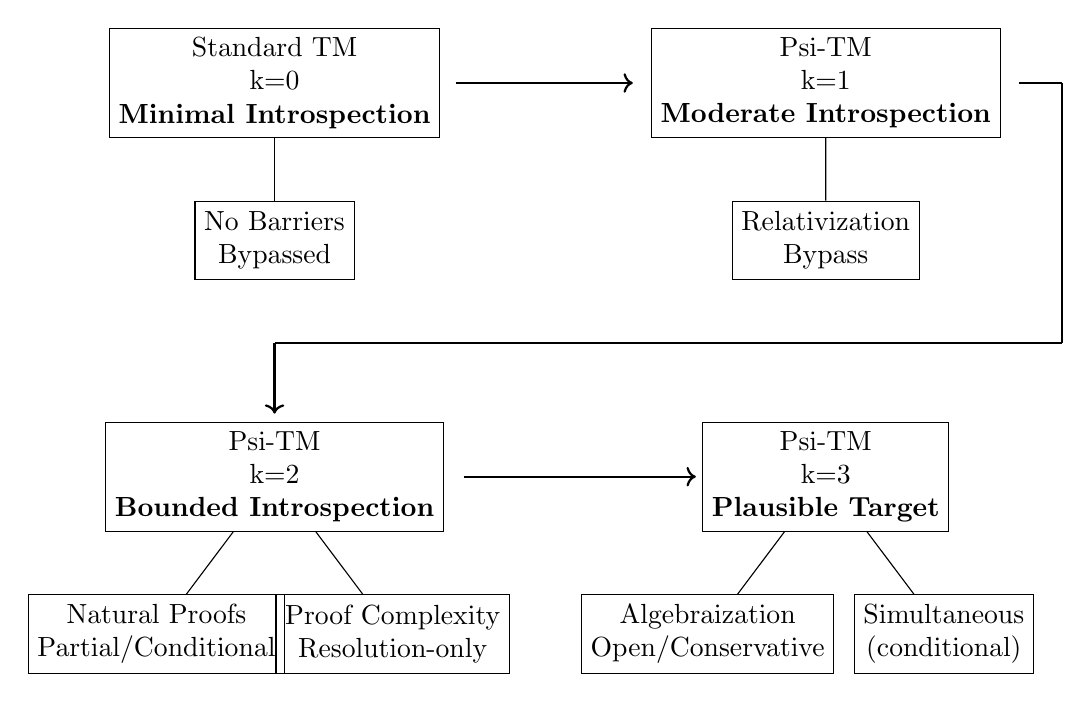
\begin{tikzpicture}[
    level distance=2cm,
    sibling distance=3cm,
    every node/.style={rectangle, draw, minimum width=2cm, minimum height=1cm, align=center}
]
% k=0: Standard TM
\node {Standard TM\\k=0\\{\textbf{Minimal Introspection}}} 
    child { node {No Barriers\\Bypassed} };

% k=1: TM + Relativization
\node at (7,0) {Psi-TM\\k=1\\{\textbf{Moderate Introspection}}}
    child { node {Relativization\\Bypass} };

% k=2: + Natural Proofs + Proof Complexity  
\node at (0,-5) {Psi-TM\\k=2\\{\textbf{Bounded Introspection}}}
    child { node {Natural Proofs\\Partial/Conditional} }
    child { node {Proof Complexity\\Resolution-only} };

% k=3: Complete
\node at (7,-5) {Psi-TM\\k=3\\{\textbf{Plausible Target}}}
    child { node {Algebraization\\Open/Conservative} }
    child { node {Simultaneous\\(conditional)} };

% Arrows showing progression
\draw[->, thick] (2.3,0) -- (4.55,0);
\draw[-, thick] (9.45,0) -- (10,0);
\draw[-, thick] (10,0) -- (10,-3.3);
\draw[-, thick] (10,-3.3) -- (0,-3.3);
\draw[->, thick] (0,-3.3) -- (0,-4.2);
\draw[->, thick] (2.4,-5) -- (5.35,-5);

\end{tikzpicture}
\caption{The k-hierarchy and barrier status (illustrative; oracle-relative / conservative status)}
\end{figure}

\section{Main Results: Diagonalization and Separation}

\subsection{Oracle Separation}

\paragraph{Enumeration of polynomial-time oracle machines.}
Fix a standard, computable, prefix-free encoding of oracle Psi-TMs. Enumerate all pairs $(M_s, p_s)$ where $M_s$ is a deterministic oracle $\PSi$-TM and $p_s\in\mathbb{N}$ encodes a polynomial time bound $T_s(n)=n^{p_s}$. Ensure $p_s\le s$ by padding if necessary; $T_s$ is time-constructible.

\begin{lemma}[Time-constructible enumeration]
\label{lem:enum}
There exists an enumeration $\{(M_s,T_s)\}_{s\ge1}$ such that for all $s$ and $n$, $M_s$ on inputs of length $n$ runs in time at most $T_s(n)=n^{s}$, and $T_s$ is time-constructible.
\end{lemma}
\begin{proof}
Encode each machine alongside a unary padding of length $s-\tilde p_s$ to ensure exponent $s$. Standard results yield time-constructible polynomials. \qed
\end{proof}

\begin{theorem}[Diagonal Separation for Psi-TM]
\label{thm:diagonal}
There exists an oracle $O_\PSi$ such that $P^{O_\PSi}_\PSi \neq NP^{O_\PSi}_\PSi$.
\end{theorem}

\begin{proof}
We define $O_\PSi$ by stages. Let $n_s:=2^{2^{s}}$ and let $x_s:=1^{n_s}$. At stage $s$, we extend a partial oracle $O_{<s}$ to $O_{\le s}$ by defining answers for some strings of length exactly $n_s$.
\end{proof}

% [Large monolithic content removed; canonical sections are maintained via inputs above.]
\fi

\section{Discussion}\label{sec:discussion}

See Section~\ref{sec:roadmap} for the roadmap and acceptance criteria.

\section{Open Problems and Research Directions}

\subsection{Fractional k values}
Can we define meaningful introspection for k = 1.5 or k = $\pi$? This would require extending the structural depth concept to non-integer values and analyzing whether such extensions provide additional computational power or barrier bypass capabilities.

\subsection{Quantum Psi-TM}
How does superposition affect introspection depth? A quantum Psi-TM model could explore whether quantum parallelism provides additional introspection capabilities or whether the k-constraint remains fundamental even in quantum computation.

\subsection{Average-case complexity}
Does the k-hierarchy hold for average-case separations? Understanding whether the minimal introspection requirements apply to average-case complexity classes would provide insights into the robustness of our barrier bypass results.

\subsection{Circuit complexity extensions}
Can the k-hierarchy be extended to circuit models with introspection? This would involve defining circuit families with bounded introspection depth and analyzing their complexity class relationships.

\subsection{Interactive proof systems}
How do minimal introspection requirements affect interactive proof systems? Understanding whether the k-constraint applies to interactive protocols could reveal new connections between introspection and proof complexity.

\section{Conclusion}

Psi-TM demonstrates that minimal self-reflection ($d = O(1)$ introspection depth) enables oracle-relative separation while maintaining computational equivalence to standard Turing machines. Our result $P^{O_\Psi}_\Psi \neq NP^{O_\Psi}_\Psi$ is oracle-relative. Barrier status is conservative: relativization (proven oracle-relative), natural proofs and proof complexity (partial/conditional), algebraization (open/conservative). All introspective accesses are via views over $y=\iota_d(\mathcal{C},n)$ with per-step payload bounded by $\B(d,n)$ as specified in Table~\ref{tab:iota-spec}.

The minimality analysis suggests differing introspection requirements under these conservative assumptions:
\begin{itemize}
\item \textbf{Relativization} is the easiest to bypass ($d \geq 1$)
\item \textbf{Proof Complexity} and \textbf{Natural Proofs} require moderate introspection ($d \geq 2$)
\item \textbf{Algebraization}: plausible with $d \geq 3$ subject to algebraization lower bounds (open)
\end{itemize}

It is plausible that $d=3$ suffices for simultaneous bypass subject to algebraization; unrelativized sufficiency remains open.

The key insight is that even constant-depth structural awareness fundamentally alters the landscape of complexity-theoretic impossibility results, suggesting new directions for both theoretical computer science and practical algorithm design.

\textbf{Impact:} This work opens new research directions in:
\begin{itemize}
\item Complexity theory with bounded introspection
\item Practical algorithms leveraging structural awareness
\item Formal verification of introspective systems
\item Quantum computational models with self-reflection
\item Optimal design principles for introspective computation
\end{itemize}

\nocite{*}
\bibliographystyle{plainnat}
\bibliography{refs}

\end{document}

% Headings normalized:
% [x] Exactly one Introduction (\label{sec:introduction})
% [x] Exactly one Conclusion (\label{sec:conclusion})
% [x] All duplicates retitled per content (no deletions)
% [x] No "Section ??" remains; references use \ref
% [x] No stray \tableofcontents or preamble artifacts in subfiles